% ============================================================================
%  PulseFinance -- SE3092 Assignment 01 Technical Report
%  Compile with pdflatex (twice, for the table of contents), e.g. on Overleaf.
% ============================================================================
\documentclass[11pt,a4paper]{article}

% ---- Fill these in before submitting ----------------------------------------
\newcommand{\IDHesara}{IT\,XXXXXXXX}
\newcommand{\IDSandali}{IT\,XXXXXXXX}
\newcommand{\IDShazaan}{IT\,XXXXXXXX}
\newcommand{\SubmissionDate}{November 2026}
% -----------------------------------------------------------------------------

\usepackage[T1]{fontenc}
\usepackage[utf8]{inputenc}
\usepackage{lmodern}
\usepackage{textcomp}
\usepackage[a4paper,margin=2.3cm,headheight=14pt]{geometry}
\usepackage[table]{xcolor}
\usepackage{tikz}
\usetikzlibrary{arrows.meta,positioning,shapes.geometric,fit,calc,backgrounds}
\usepackage{booktabs,longtable,tabularx,array,multirow}
\usepackage{enumitem}
\usepackage{caption}
\usepackage{float}
\usepackage{pdflscape}
\usepackage{listings}
\usepackage{fancyhdr}
\usepackage{titlesec}
\usepackage{amsmath,amssymb}
\usepackage[hidelinks]{hyperref}

% ---- Colours from ui/theme/Color.kt ------------------------------------------
\definecolor{pfgreen}{HTML}{00C950}
\definecolor{pfgreendark}{HTML}{006E28}
\definecolor{pfgreenlight}{HTML}{E6F9EC}
\definecolor{pfamber}{HTML}{F59E0B}
\definecolor{pfamberdark}{HTML}{B45309}
\definecolor{pfamberlight}{HTML}{FEF3C7}
\definecolor{pfsurface}{HTML}{F7F9FB}
\definecolor{pfborder}{HTML}{E2E8F0}
\definecolor{pftext}{HTML}{191C1E}
\definecolor{pfmuted}{HTML}{565E74}
\definecolor{pfblue}{HTML}{3B82F6}
\definecolor{pfviolet}{HTML}{8B5CF6}
\definecolor{pforange}{HTML}{F97316}

% ---- Layout -----------------------------------------------------------------
\setlength{\parskip}{0.55em}
\setlength{\parindent}{0pt}
\renewcommand{\arraystretch}{1.25}
\setlist{itemsep=0.15em,topsep=0.3em}
\captionsetup{font=small,labelfont={bf,color=pfgreendark}}

\titleformat{\section}{\Large\bfseries\sffamily\color{pfgreendark}}{\thesection}{0.8em}{}
\titleformat{\subsection}{\large\bfseries\sffamily\color{pftext}}{\thesubsection}{0.7em}{}
\titleformat{\subsubsection}{\normalsize\bfseries\sffamily\color{pftext}}{\thesubsubsection}{0.6em}{}

\pagestyle{fancy}
\fancyhf{}
\fancyhead[L]{\small\sffamily\color{pfmuted}PulseFinance -- SE3092 Assignment 01}
\fancyhead[R]{\small\sffamily\color{pfmuted}\leftmark}
\fancyfoot[C]{\small\sffamily\thepage}
\renewcommand{\headrulewidth}{0.4pt}

\lstset{basicstyle=\ttfamily\footnotesize,columns=fullflexible,keepspaces=true,
  frame=single,rulecolor=\color{pfborder},backgroundcolor=\color{pfsurface},
  xleftmargin=0.6em,xrightmargin=0.6em,framexleftmargin=0.4em,breaklines=true,
  aboveskip=0.8em,belowskip=0.6em}

% ---- Helpers ----------------------------------------------------------------
% \code: monospaced text typeset literally, with line breaks allowed after / . _ - and inside camelCase
\ExplSyntaxOn
\tl_new:N \l__pf_code_tl
\NewDocumentCommand{\code}{m}
 {
  \texttt
   {
    \tl_set:Nx \l__pf_code_tl { \tl_to_str:n {#1} }
    \regex_replace_all:nnN { ([/._\-]) } { \1 \c{allowbreak} } \l__pf_code_tl
    \regex_replace_all:nnN { ([a-z])([A-Z]) } { \1 \c{allowbreak} \2 } \l__pf_code_tl
    \l__pf_code_tl
   }
 }
\ExplSyntaxOff
\emergencystretch=3em
\newcommand{\req}[1]{\textsf{\textbf{\color{pfgreendark}#1}}}
\newcommand{\prob}[1]{\textsf{\textbf{\color{pfamberdark}#1}}}
\newcommand{\lkr}[1]{LKR~#1}
\newcommand{\status}[1]{\textsf{\small #1}}
\newcolumntype{L}{>{\raggedright\arraybackslash}X}
\newcolumntype{C}[1]{>{\centering\arraybackslash}p{#1}}

% A numbered callout used in the wireframes and their legends
\newcommand{\callout}[1]{\tikz[baseline=(c.base)]\node[circle,fill=pfamber,text=white,
  font=\sffamily\bfseries\scriptsize,inner sep=1.2pt,minimum size=12pt](c){#1};}

\tikzset{
  phone/.style={draw=pftext,line width=1.2pt,rounded corners=10pt,fill=pfsurface},
  card/.style={draw=pfborder,fill=white,rounded corners=4pt,line width=0.6pt},
  hero/.style={fill=pfgreen,rounded corners=5pt,draw=none},
  chip/.style={draw=pfborder,fill=white,rounded corners=3pt,font=\sffamily\tiny,inner sep=2pt},
  chipon/.style={draw=pfgreendark,fill=pfgreenlight,rounded corners=3pt,font=\sffamily\tiny,inner sep=2pt},
  warn/.style={fill=pfamberlight,draw=pfamber,rounded corners=4pt,line width=0.6pt},
  wftext/.style={font=\sffamily\tiny,text=pftext,align=left,anchor=west},
  wfmuted/.style={font=\sffamily\tiny,text=pfmuted,align=left,anchor=west},
  num/.style={circle,fill=pfamber,text=white,font=\sffamily\bfseries\scriptsize,inner sep=1pt,minimum size=12pt},
  layer/.style={draw=#1,fill=#1!8,rounded corners=4pt,line width=0.8pt,font=\sffamily\small},
  box/.style={draw=#1,fill=#1!10,rounded corners=3pt,font=\sffamily\scriptsize,align=center,
    minimum width=2.9cm,minimum height=0.62cm,inner sep=2pt},
  arr/.style={-{Stealth[length=2mm]},draw=pfmuted,line width=0.5pt},
}

% Phone frame: \phoneframe{title}
\newcommand{\phoneframe}[1]{%
  \draw[phone] (0,0) rectangle (6,12);
  \fill[pftext] (2.4,11.78) rectangle (3.6,11.86);
  \node[font=\sffamily\scriptsize\bfseries,text=pftext,anchor=west] at (0.35,11.35) {#1};
  \draw[pfborder] (0.2,11.0) -- (5.8,11.0);
}
% Bottom dock with the current tab highlighted: \dock{index 1..5}
\newcommand{\dock}[1]{%
  \draw[card] (0.35,0.25) rectangle (5.65,1.05);
  \foreach \i/\lab in {1/Today,2/Analytics,3/Income,4/Quest,5/Audit}{
    \pgfmathsetmacro{\x}{0.35+(\i-0.5)*1.06}
    \ifnum\i=#1
      \fill[pfgreenlight] (\x,0.66) circle (0.26);
    \fi
    \ifnum\i=3
      \draw[pfgreen,line width=0.8pt,fill=white] (\x,0.72) circle (0.26);
    \else
      \draw[pfmuted,line width=0.5pt] (\x-0.1,0.6) rectangle (\x+0.1,0.8);
    \fi
    \node[font=\sffamily\fontsize{4.5}{5}\selectfont,text=pfmuted] at (\x,0.38) {\lab};
  }
}

\hypersetup{pdftitle={PulseFinance -- Technical Report},pdfauthor={Hesara, Sandali, Shazaan}}

% ============================================================================
\begin{document}

% ---- Title page -------------------------------------------------------------
\begin{titlepage}
\thispagestyle{empty}
\begin{tikzpicture}[remember picture,overlay]
  \fill[pfgreen] (current page.north west) rectangle ([yshift=-7.2cm]current page.north east);
  \fill[pfgreendark] ([yshift=-7.2cm]current page.north west) rectangle ([yshift=-7.5cm]current page.north east);
\end{tikzpicture}

\vspace*{0.4cm}
{\color{white}\sffamily
{\large SE3092 Platform Based Development \textperiodcentered{} Assignment 01}\\[1.2cm]
{\fontsize{38}{42}\selectfont\bfseries PulseFinance}\\[0.4cm]
{\Large A personal finance app for one person's real financial life}\par}

\vspace{2.6cm}
{\sffamily\large\bfseries\color{pftext} Technical Report}\\[0.2cm]
{\sffamily\color{pfmuted} Requirements analysis \textperiodcentered{} Firestore schema \textperiodcentered{} MVVM architecture \textperiodcentered{} Annotated wireframes \textperiodcentered{} Design decisions}

\vspace{1.4cm}
\begin{tabular}{@{}p{4.2cm}p{4cm}@{}}
\toprule
\sffamily\bfseries Team member & \sffamily\bfseries Student ID\\
\midrule
Hesara Perera & \IDHesara\\
Sandali & \IDSandali\\
Shazaan & \IDShazaan\\
\bottomrule
\end{tabular}

\vfill
\begin{tabularx}{\textwidth}{@{}lL@{}}
\sffamily\bfseries Built for & Kavindu Silva, 25, junior software engineer, Colombo\\
\sffamily\bfseries Platform & Android 8.0+ (minSdk 26, targetSdk 34), Kotlin, Jetpack Compose\\
\sffamily\bfseries Backend & Firebase Authentication, Cloud Firestore (\code{finance-app-se3092})\\
\sffamily\bfseries Repository & \code{github.com/Hesara2003/PulseFinance-SE3092}\\
\sffamily\bfseries Date & \SubmissionDate\\
\end{tabularx}
\end{titlepage}

% ---- Summary + contents -----------------------------------------------------
\pagenumbering{roman}
\section*{Summary}
\addcontentsline{toc}{section}{Summary}
Kavindu Silva earned more than \lkr{1.6 million} in twelve months and has \lkr{11,200} left. His money arrives four ways: a salary that lands on the 25th, freelance milestones he sometimes forgets to chase, Google AdSense paid in US dollars at whatever rate his bank applies, and crypto trades that gained in Q1 and lost in Q3. It leaves through his card, cash, PickMe and UberEats, and a secondary account that auto-debits a gym and two subscriptions he meant to cancel six months ago. He wants a MacBook Pro M4, about \lkr{490,000}, within a year. He has tried four tools -- a Google Sheet, a Play Store budget app, a Notes file and his bank's own summary -- and abandoned all four.

This report argues that the problem was never discipline. \emph{None of those tools could represent his financial life accurately enough to be worth maintaining.} PulseFinance is designed against each of those four failures. It records income at the amount actually received and freezes the exchange rate with it; it keeps unpaid invoices out of what he can spend; it captures cash and secondary-account spending through presets and shared bank SMS; it surfaces forgotten subscriptions from his own charges; and it turns the MacBook into a required daily pace that it compares with what he really saves.

The report covers the requirements analysis (Section~\ref{sec:requirements}), the MVVM architecture (Section~\ref{sec:architecture}), the Firestore schema (Section~\ref{sec:schema}), annotated wireframes of every main screen (Section~\ref{sec:wireframes}) and the justification of sixteen design decisions (Section~\ref{sec:decisions}). Every requirement, field and screen element is traced back to a specific part of Kavindu's scenario. At the time of writing, 69 of the 73 requirements are implemented; the four that are not are listed with their gaps in Section~\ref{sec:status}.

\tableofcontents
\clearpage
\pagenumbering{arabic}

% ============================================================================
\section{Introduction}
\label{sec:intro}

\subsection{Purpose and scope}
PulseFinance is a native Android application that gives one person an honest monthly picture of three things:
\begin{itemize}
  \item \textbf{income} from four irregular, multi-currency sources;
  \item \textbf{spending}, split by whether he had to make it (committed) or chose to (discretionary);
  \item \textbf{progress towards one quantified goal}: the MacBook Pro M4.
\end{itemize}
It does this without importing anything from a bank (constraint C-12). Kavindu remains the source of truth, so the whole design optimises for three properties: recording must be fast, missing records must never feel like failure, and the numbers must be trustworthy enough that he keeps opening the app.

\subsection{How this report is organised}
\begin{tabularx}{\textwidth}{@{}lL@{}}
\toprule
\textbf{Section} & \textbf{Content}\\
\midrule
\ref{sec:requirements} Requirements analysis & Scenario analysis, failed-tool analysis, problem statements, 73 requirements with status, constraints, traceability\\
\ref{sec:architecture} Architecture & Layers, the MVVM diagram, offline-first data flow, dependency injection\\
\ref{sec:schema} Firestore schema & Collections, fields with Kavindu's data as examples, rules, local cache, ER model\\
\ref{sec:wireframes} Annotated wireframes & Six screens, each element tied to a problem and a requirement\\
\ref{sec:decisions} Design decisions & Sixteen decisions with context, alternatives and consequences\\
\ref{sec:status} Implementation status & Testing, delivery, open gaps, team contributions\\
\bottomrule
\end{tabularx}

Requirement identifiers (\req{FR-INC-6}, \req{NFR-2}, \ldots) and problem identifiers (\prob{P1}--\prob{P11}) are used throughout so that any claim can be traced to the requirements in Section~\ref{sec:requirements} and to the source code. The full Software Requirements Specification is in the repository at \code{docs/SRS.md}.

% ============================================================================
\section{Requirements Analysis}
\label{sec:requirements}

\subsection{Kavindu's situation}
\begin{tabularx}{\textwidth}{@{}p{3.4cm}L@{}}
\toprule
\textbf{Aspect} & \textbf{What the scenario tells us}\\
\midrule
Who & 25, junior software engineer in Colombo; comfortable with technology, low tolerance for friction in daily data entry.\\
Income & Salary (credited on the 25th); freelance web projects paid in milestones; Google AdSense in USD, credited in LKR at the bank's rate; crypto trading with a significant Q1 gain and a material Q3 loss. His own estimate of monthly income, ``LKR 160,000--210,000'', has never been validated.\\
Spending & Card, cash, PickMe, UberEats; rent \lkr{34,000}; a gym membership and two subscriptions auto-debited from a secondary account he rarely checks. Discovering ``LKR 24,000 on coffee'' was ``genuinely shocking''.\\
Savings & More than \lkr{1.6 million} earned in twelve months; \lkr{11,200} saved.\\
Goal & MacBook Pro M4 from an authorised reseller, about \lkr{490,000}, within 12 months. ``Emotionally present and financially invisible.''\\
Behaviour & Optimistic about income, impulsive with discretionary spending, avoids looking at money when worried, and abandons tools once their numbers stop matching reality.\\
\bottomrule
\end{tabularx}

\subsection{Why four tools failed}
The most useful evidence in the scenario is the list of tools Kavindu has already given up on. Each failure points to a property PulseFinance must have.

\begin{tabularx}{\textwidth}{@{}p{0.6cm}p{2.5cm}LL@{}}
\toprule
\textbf{ID} & \textbf{Tool} & \textbf{Why it failed} & \textbf{What PulseFinance does instead}\\
\midrule
F1 & Google Sheet ``MacBook Fund'' & Formulas broke when rows were inserted; entry was slow; after a three-week gap the incomplete rows felt discouraging. & All calculation lives in tested domain use cases, not editable formulas. Days without records are missing data, never zero or failure (\req{NFR-2}).\\
F2 & Play Store budget app & USD only; no cloud sync; assumed one income source and a fixed monthly budget. & Income Source is a first-class concept; each entry keeps its original currency and the rate actually received; the allowance is recalculated daily (\req{FR-INC-1}, \req{FR-DASH-1}, \req{FR-AUTH-3}).\\
F3 & Notes app & Pasted figures became an unreadable block after four days. & Every record is captured with structure -- category, committed or discretionary, account -- at entry time, through one-tap presets (\req{FR-EXP-1}, \req{FR-EXP-3}).\\
F4 & Bank's spending summary & Card only; missed cash and the secondary account; filed a PickMe fare as ``online retail''. & Accounts include cash, the secondary account and the crypto exchange; the category only \emph{suggests} committed or discretionary and Kavindu decides (\req{FR-ACC-1}, \req{FR-EXP-2}).\\
\bottomrule
\end{tabularx}

The common root cause is that each tool was \textbf{too fragile, too manual, too narrow or too unpleasant to open}. Each of those maps to a non-functional requirement: fragile to \req{NFR-6}, manual to \req{NFR-1}, narrow to the \req{FR-INC} group, unpleasant to \req{NFR-2} and \req{NFR-8}.

\subsection{Problem statements}
\begin{tabularx}{\textwidth}{@{}p{0.7cm}L@{}}
\toprule
\textbf{ID} & \textbf{Problem}\\
\midrule
\prob{P1} & He cannot state his real monthly income; the estimate ``LKR 160,000--210,000'' was never validated.\\
\prob{P2} & Freelance invoices are forgotten and payments cannot be matched to projects.\\
\prob{P3} & AdSense income in USD is never recorded at the amount actually received.\\
\prob{P4} & He has no running net crypto position and cannot answer ``what did crypto earn me this year?''.\\
\prob{P5} & Spending is spread across card, cash, PickMe, UberEats and a secondary auto-debit account, with no single view.\\
\prob{P6} & Two subscriptions he meant to cancel six months ago are still being charged.\\
\prob{P7} & He has no idea of his committed versus discretionary split and has never seen how his spending is distributed.\\
\prob{P8} & He does not know the monthly saving needed for \lkr{490,000} in 12 months, because he does not know what he currently saves.\\
\prob{P9} & Gaps in tracking made his previous tool feel discouraging and led to abandonment.\\
\prob{P10} & He does not examine his payslip and cannot recall the amount deposited.\\
\prob{P11} & He is impulsive with discretionary spending and has no friction at the point of purchase.\\
\bottomrule
\end{tabularx}

\subsection{Analytical lenses}
\paragraph{What must the system understand about his income?} A single ``income'' number hides four things: the \emph{source} (salary, freelance, AdSense, crypto); whether the money is \emph{realised or only invoiced} -- a pending invoice is not spendable; the \emph{original currency and the rate actually received} -- AdSense is credited at the bank's rate, not the market rate; and the \emph{sign} -- a crypto loss is negative income. Timing matters too: because the salary lands on the 25th, ``income so far this month'' is misleading for most of the month. The daily allowance is therefore based on an \textbf{Income Basis}: the higher of this month's realised income and the average of the previous three months, with crypto \emph{profits} excluded from that average so that one lucky trade cannot inflate the allowance of an income-optimistic, impulsive spender (\req{FR-DASH-3}).

\paragraph{What must the system understand about his spending?} Whether each expense was \emph{committed} (rent, utilities, subscriptions) or \emph{discretionary} (coffee, PickMe, dining), which \emph{account} it came from, and whether a recurring charge is something he still uses. The bank summary failed because it guessed the category and saw only one card; PulseFinance proposes, he decides, and every account he uses is in scope.

\paragraph{What feedback makes a goal feel real?} A goal becomes actionable when it is expressed in the same units as his daily choices: a required daily pace (about \lkr{1,330} per day), a comparison with what he actually saves, an arrival date, and the cost of a habit in ``days of MacBook''. Progress must only ever move forward -- no streaks to break.

\subsection{Functional requirements}
Priorities use MoSCoW (M, S, C). Status reflects the code on \code{main} at the time of writing.

\begin{longtable}{@{}p{2.2cm}p{9.5cm}C{0.7cm}p{1.6cm}@{}}
\toprule
\textbf{ID} & \textbf{Requirement} & \textbf{Pri} & \textbf{Status}\\
\midrule
\endfirsthead
\toprule
\textbf{ID} & \textbf{Requirement} & \textbf{Pri} & \textbf{Status}\\
\midrule
\endhead
\multicolumn{4}{@{}l}{\textbf{\textsf{Identity and onboarding}}}\\
FR-AUTH-1 & Register and sign in with email and password (Firebase Authentication). & M & Done\\
FR-AUTH-2 & Sign in with a Google account. & S & Done\\
FR-AUTH-3 & Every record stored under the signed-in user's ID, so the same data appears on any device. & M & Done\\
FR-AUTH-4 & First-run setup captures salary, active Income Sources and fixed monthly commitments (e.g.\ rent \lkr{34,000}) in three steps. & M & Done\\
FR-AUTH-5 & Setup records each source's expected variability (steady, varies, highly volatile). & C & Done\\
FR-AUTH-6 & Setup lets him set an emergency-runway buffer of 1--6 months of committed costs; the dashboard shows its size and his progress. & C & Done\\
FR-AUTH-7 & A debug-only demo drawer fills credentials for a pre-seeded account; credentials come from build configuration. & M & Done\\
\multicolumn{4}{@{}l}{\textbf{\textsf{Income}}}\\
FR-INC-1 & Each entry records source, title, client or platform, original amount, currency (LKR, USD, USDT, ETH) and date. & M & Done\\
FR-INC-2 & The exchange rate used is stored with the entry and never recomputed (ADR-0001). & M & Done\\
FR-INC-3 & Freelance income can be a Pending Invoice with client and due date, marked received in one tap. & M & Done\\
FR-INC-4 & A pending invoice past its due date is automatically treated as overdue. & M & Done\\
FR-INC-5 & The form pre-fills the day's suggested rate (open.er-api.com, CoinGecko), cached daily, usable offline with its age shown. & M & Done\\
FR-INC-6 & For a foreign-currency entry he can type the LKR his bank actually credited; the effective rate is derived and stored. & M & Done\\
FR-INC-7 & A crypto trade is a Crypto Trading Result: positive for a profit, negative for a loss. & M & Done\\
FR-INC-8 & The Crypto year-to-date net is shown. & M & Done\\
FR-INC-9 & Realised income and pending/overdue amounts are shown separately for the month, by source. & M & Done\\
\multicolumn{4}{@{}l}{\textbf{\textsf{Expenses}}}\\
FR-EXP-1 & Each expense records amount (LKR), category, committed/discretionary flag, account, time and note. & M & Done\\
FR-EXP-2 & The category proposes committed or discretionary; he can flip it in one tap. & M & Done\\
FR-EXP-3 & One-tap Sri Lankan presets (coffee, PickMe, UberEats, rent). & M & Done\\
FR-EXP-4 & Presets include Dialog and Mobitel reloads and data packages. & S & Done\\
FR-EXP-5 & Expenses can be attributed to any account, including cash and the secondary auto-debit account. & M & Done\\
FR-EXP-6 & An expense saved offline appears immediately and syncs on reconnection. & M & Done\\
FR-EXP-7 & A bank SMS shared through the share sheet becomes a draft expense (amount, merchant, card last four digits), without READ\_SMS. & S & Done\\
\multicolumn{4}{@{}l}{\textbf{\textsf{Subscriptions}}}\\
FR-SUB-1 & Recurring subscriptions are detected by grouping subscription-category expenses by merchant over 120 days. & M & Done\\
FR-SUB-2 & Each shows its monthly and annual cost and the account it is charged to. & M & Done\\
FR-SUB-3 & He records Keep or Cancel; a charge after Cancel flags it as ``still charging''. & M & Done\\
FR-SUB-4 & After a charge: ``Did you use this this month?''; two consecutive Nos set the risk to High. & S & Done\\
FR-SUB-5 & For app-linked subscriptions (Netflix, Spotify), usage statistics show when the app was last opened and feed the risk. & S & Partial\\
FR-SUB-6 & Results are grouped by account, with the secondary account highlighted. & S & Done\\
\multicolumn{4}{@{}l}{\textbf{\textsf{Savings goal}}}\\
FR-GOAL-1 & Set a goal with title, LKR target and date (for Kavindu: MacBook Pro M4, \lkr{490,000}, 12 months). & M & Done\\
FR-GOAL-2 & The required monthly and daily saving is calculated. & M & Done\\
FR-GOAL-3 & The actual savings rate is calculated (realised income minus spending, over 90 days or since the first record). & M & Done\\
FR-GOAL-4 & The arrival date is projected at the actual rate, stating whether he is on pace or behind, and by how much. & M & Done\\
FR-GOAL-5 & Any amount can be translated into ``days of goal funded'' (opportunity cost). & S & Done\\
FR-GOAL-6 & An optional USD reference price makes the LKR target follow the daily rate; the change is shown. & S & Done\\
FR-GOAL-7 & Quick-add boosters (+\lkr{5,000} / 10,000 / 25,000) move a windfall into the goal. & C & Done\\
\multicolumn{4}{@{}l}{\textbf{\textsf{Dashboard}}}\\
FR-DASH-1 & Safe-to-Spend Allowance per day for the rest of the month. & M & Done\\
FR-DASH-2 & Pending and overdue invoices are never counted as spendable. & M & Done\\
FR-DASH-3 & The three-month average in the Income Basis excludes crypto profits but keeps crypto losses. & M & Done\\
FR-DASH-4 & The month's committed versus discretionary split as a bar with amounts. & M & Done\\
FR-DASH-5 & An overdue-invoice banner with client and amount and one-tap ``mark received''. & M & Done\\
FR-DASH-6 & Figures update in real time from Firestore listeners. & M & Done\\
\multicolumn{4}{@{}l}{\textbf{\textsf{Analytics and data}}}\\
FR-ANA-1 & Category donut for the period, discretionary distinguishable from committed. & M & Done\\
FR-ANA-2 & Week and month periods. & M & Done\\
FR-ANA-3 & Daily spending bars with the peak day highlighted. & S & Done\\
FR-ANA-4 & Day and year periods. & C & Done\\
FR-ANA-5 & Transactions searchable by keyword and filterable by account, category and date. & C & Done\\
FR-DATA-1 & Export all income, expenses and goals to CSV. & S & Done\\
\multicolumn{4}{@{}l}{\textbf{\textsf{Accounts and Spending Freeze}}}\\
FR-ACC-1 & Accounts of type Primary Bank, Secondary Bank (auto-debit), Cash and Crypto Exchange. & M & Done\\
FR-ACC-2 & Combined balance across his recorded accounts. & S & Done\\
FR-ACC-3 & A Spending Freeze on an account until a chosen date; the account shows as locked. & S & Done\\
FR-ACC-4 & Spending from a frozen account shows the cost in goal days and offers ``Log anyway''; recording is never refused. & S & Done\\
FR-ACC-5 & Freeze Breaks are counted and shown. & S & Done\\
FR-ACC-6 & Account numbers masked (\textbullet\textbullet\textbullet\textbullet{} 4521), revealed only after biometric or device-PIN authentication. & S & Done\\
FR-ACC-7 & A revealed number can be copied for a freelance invoice; the clipboard is cleared after 60 seconds. & S & Done\\
\multicolumn{4}{@{}l}{\textbf{\textsf{Sri Lankan context}}}\\
FR-LK-1 & Payslip: gross salary to employee EPF (8\%), APIT and take-home; all editable. & M & Done\\
FR-LK-2 & APIT tax bands read from Firestore configuration, not compiled into the app. & M & Done\\
FR-LK-3 & Accumulating EPF balance (employee 8\% + employer 12\%) shown as savings he owns. & S & Done\\
FR-LK-4 & Seasonal Peaks (Avurudu, Vesak, Poson, December) plus, after 12 months, his own months $\geq$20\% above average. & S & Done\\
FR-LK-5 & 30 days before a peak: a warning with last year's excess and a one-tap ``set aside''. & S & Done\\
FR-LK-6 & Amounts in LKR with separators; foreign amounts show the original currency beside the LKR value. & M & Done\\
\bottomrule
\end{longtable}

\subsection{Non-functional requirements}
\begin{longtable}{@{}p{1.5cm}p{2.5cm}p{5.0cm}p{2.9cm}p{1.5cm}@{}}
\toprule
\textbf{ID} & \textbf{Quality} & \textbf{Requirement} & \textbf{Measurable target} & \textbf{Status}\\
\midrule
\endfirsthead
\toprule
\textbf{ID} & \textbf{Quality} & \textbf{Requirement} & \textbf{Measurable target} & \textbf{Status}\\
\midrule
\endhead
NFR-1 & Capture speed & Logging a preset expense is fast enough to do at the point of purchase. & $\leq$3 taps, $\leq$5 s & Done\\
NFR-2 & Gap tolerance & Logging gaps are never shown as zero spending, broken streaks or failure; averages only over periods with data. & No penalty, streak reset or ``0 spent'' for unrecorded days & Partial\\
NFR-3 & Offline & All screens work offline from cached data; offline writes sync on reconnection. & Sync $\leq$10 s after reconnection & Done\\
NFR-4 & Real-time & Changes from another device appear without a refresh. & $\leq$2 s online & Done\\
NFR-5 & Data isolation & Each user can access only \code{users/{uid}}, enforced by Firestore rules. & No cross-user access & Done\\
NFR-6 & Financial accuracy & Original amount, currency and rate kept per income entry; totals derivable from stored records. & Totals unchanged after a rate change & Done\\
NFR-7 & Compatibility & Installs and runs on Android 8.0+, starts quickly. & minSdk 26, targetSdk 34 & Done\\
NFR-8 & Accessibility & Status never by colour alone; text usable at large font sizes. & Icon or label per status; 200\% font scale & Planned\\
NFR-9 & Robustness & No screen crashes or appears blank with no data, partial data or a network error. & Designed empty state everywhere & Done\\
NFR-10 & Sensitive display & Account numbers masked by default, revealed only after a biometric check. & Clipboard cleared $\leq$60 s & Done\\
NFR-11 & Portability & Data exportable in an open format. & CSV opens in Sheets/Excel & Done\\
NFR-12 & Privacy & Minimum permissions; optional ones requested in context with an explanation. & No READ\_SMS; usage access in context & Partial\\
\bottomrule
\end{longtable}

\subsection{Constraints}
\begin{tabularx}{\textwidth}{@{}p{1cm}L@{}}
\toprule
\textbf{ID} & \textbf{Constraint}\\
\midrule
C-1--C-7 & 100\% Kotlin; Jetpack Compose with Material 3; MVVM with no business logic in Composables; single activity with Navigation Compose; state as \code{StateFlow}; coroutines in \code{viewModelScope}; Hilt for dependency injection.\\
C-8, C-9 & Firebase Authentication for identity; Cloud Firestore as the primary persistence layer, with \code{firestore.rules} submitted.\\
C-10, C-11 & minSdk 26, targetSdk $\geq$34; the submitted APK connects to a live Firebase project.\\
C-12, C-13 & No bank connection. Every balance and transaction is Kavindu's own record; ``freeze'' is a self-commitment, not a card block.\\
C-14 & Card CVVs are never stored, displayed or requested.\\
C-15 & READ\_SMS is not used; bank SMS enter only through the share sheet.\\
C-16 & Tax rules (APIT bands, EPF rates) are data, not code.\\
C-17 & Exchange-rate services are free third parties: called at most once a day, and the app keeps working without them.\\
C-18 & Demo credentials only in debug builds, through build configuration.\\
\bottomrule
\end{tabularx}

\subsection{Out of scope}
\begin{tabularx}{\textwidth}{@{}p{4.6cm}L@{}}
\toprule
\textbf{Item} & \textbf{Reason}\\
\midrule
Bank-feed import / open banking & Excluded by the brief (C-12); no Sri Lankan open-banking API available.\\
Real card blocking, CVV display & No bank integration (C-13); CVV storage forbidden (C-14).\\
Live crypto portfolio valuation & His question is realised year-to-date earnings (\prob{P4}); live prices add noise, not clarity.\\
Several goals competing for money & One quantified goal is the scenario's focus; the model allows more goals but no allocation logic between them.\\
Geofenced gym-usage detection & Battery and privacy cost far outweigh the benefit; the charge-day question (\req{FR-SUB-4}) covers the need.\\
Sinhala/Tamil UI, ``lakhs'' formatting & Kavindu works in English and reads LKR in thousands; deferred.\\
\bottomrule
\end{tabularx}

\subsection{Traceability: problems to requirements}
\begin{tabularx}{\textwidth}{@{}p{5.2cm}L@{}}
\toprule
\textbf{Problem} & \textbf{Requirements that address it}\\
\midrule
\prob{P1} Unknown real income & FR-INC-1, FR-INC-9, FR-DASH-1, FR-LK-1, FR-AUTH-4\\
\prob{P2} Forgotten invoices & FR-INC-3, FR-INC-4, FR-DASH-5, FR-ANA-5, FR-ACC-7\\
\prob{P3} AdSense not recorded as received & FR-INC-2, FR-INC-5, FR-INC-6, NFR-6\\
\prob{P4} No net crypto position & FR-INC-7, FR-INC-8, FR-DASH-3\\
\prob{P5} Fragmented spending channels & FR-EXP-5, FR-EXP-7, FR-ACC-1, FR-ACC-2\\
\prob{P6} Forgotten subscriptions & FR-SUB-1 to FR-SUB-6\\
\prob{P7} No committed/discretionary view & FR-EXP-2, FR-DASH-4, FR-ANA-1, FR-ANA-2\\
\prob{P8} Unknown required saving rate & FR-GOAL-2, FR-GOAL-3, FR-GOAL-4, FR-GOAL-6\\
\prob{P9} Gaps cause abandonment & NFR-1, NFR-2, NFR-9, FR-DATA-1\\
\prob{P10} Payslip not understood & FR-LK-1, FR-LK-2, FR-LK-3\\
\prob{P11} Impulsive spending & FR-ACC-3 to FR-ACC-5, FR-GOAL-5, FR-LK-4, FR-LK-5\\
\bottomrule
\end{tabularx}

% ============================================================================
\section{Architecture}
\label{sec:architecture}

\subsection{Layers}
PulseFinance is a single-activity Compose app following MVVM with a domain layer (C-3). Dependencies point inwards: screens depend on ViewModels, ViewModels on use cases and repository interfaces, and the data layer implements those interfaces. Figure~\ref{fig:layers} shows the layers; Figure~\ref{fig:mvvm} on the following page shows every screen, ViewModel, use case, repository and data source.

\begin{figure}[H]
\centering
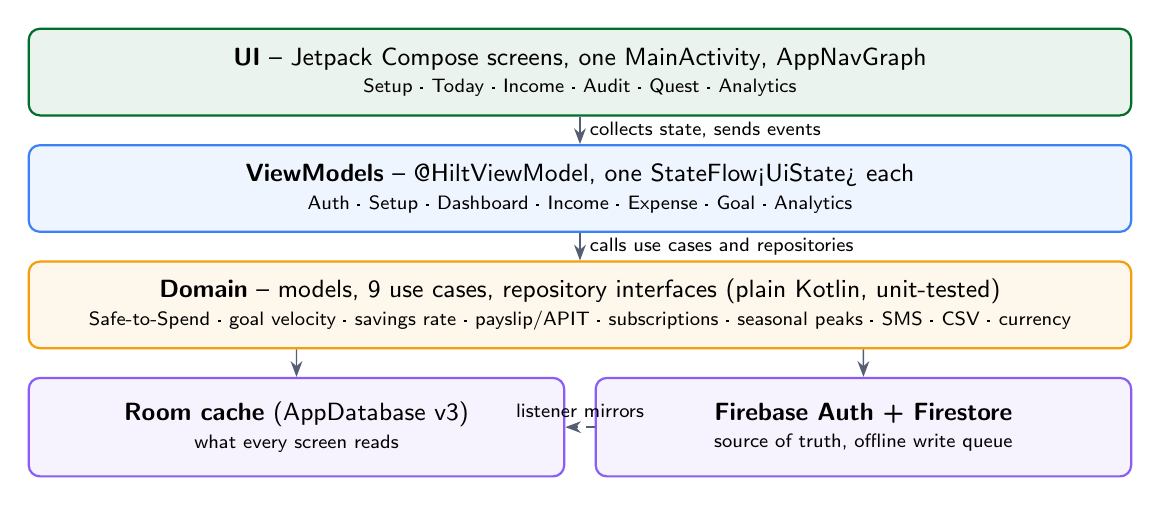
\begin{tikzpicture}[node distance=0.35cm]
\node[layer=pfgreendark,minimum width=14cm,minimum height=1.1cm,align=center] (ui)
  {\textbf{UI} -- Jetpack Compose screens, one \code{MainActivity}, \code{AppNavGraph}\\[-1pt]
   \scriptsize Setup \textperiodcentered{} Today \textperiodcentered{} Income \textperiodcentered{} Audit \textperiodcentered{} Quest \textperiodcentered{} Analytics};
\node[layer=pfblue,minimum width=14cm,minimum height=1.1cm,align=center,below=of ui] (vm)
  {\textbf{ViewModels} -- \code{@HiltViewModel}, one \code{StateFlow<UiState>} each\\[-1pt]
   \scriptsize Auth \textperiodcentered{} Setup \textperiodcentered{} Dashboard \textperiodcentered{} Income \textperiodcentered{} Expense \textperiodcentered{} Goal \textperiodcentered{} Analytics};
\node[layer=pfamber,minimum width=14cm,minimum height=1.1cm,align=center,below=of vm] (dom)
  {\textbf{Domain} -- models, 9 use cases, repository interfaces (plain Kotlin, unit-tested)\\[-1pt]
   \scriptsize Safe-to-Spend \textperiodcentered{} goal velocity \textperiodcentered{} savings rate \textperiodcentered{} payslip/APIT \textperiodcentered{} subscriptions \textperiodcentered{} seasonal peaks \textperiodcentered{} SMS \textperiodcentered{} CSV \textperiodcentered{} currency};
\node[layer=pfviolet,minimum width=6.8cm,minimum height=1.25cm,align=center,below=of dom,xshift=-3.6cm] (local)
  {\textbf{Room cache} (\code{AppDatabase} v3)\\[-1pt]\scriptsize what every screen reads};
\node[layer=pfviolet,minimum width=6.8cm,minimum height=1.25cm,align=center,below=of dom,xshift=3.6cm] (remote)
  {\textbf{Firebase Auth + Firestore}\\[-1pt]\scriptsize source of truth, offline write queue};
\draw[arr] (ui) -- node[right,font=\sffamily\scriptsize]{collects state, sends events} (vm);
\draw[arr] (vm) -- node[right,font=\sffamily\scriptsize]{calls use cases and repositories} (dom);
\draw[arr] (dom.south) ++(-3.6,0) -- (local);
\draw[arr] (dom.south) ++(3.6,0) -- (remote);
\draw[arr,dashed] (remote.west) -- node[above,font=\sffamily\scriptsize]{listener mirrors} (local.east);
\end{tikzpicture}
\caption{Layers of PulseFinance. Arrows show dependency and data direction.}
\label{fig:layers}
\end{figure}

\subsection{MVVM diagram}
Figure~\ref{fig:mvvm} is drawn from the constructors of the ViewModels on \code{main}. Every ViewModel also injects \code{AuthRepository} to obtain the signed-in user's ID; that link is omitted for readability.

\begin{landscape}
\begin{figure}[p]
\centering
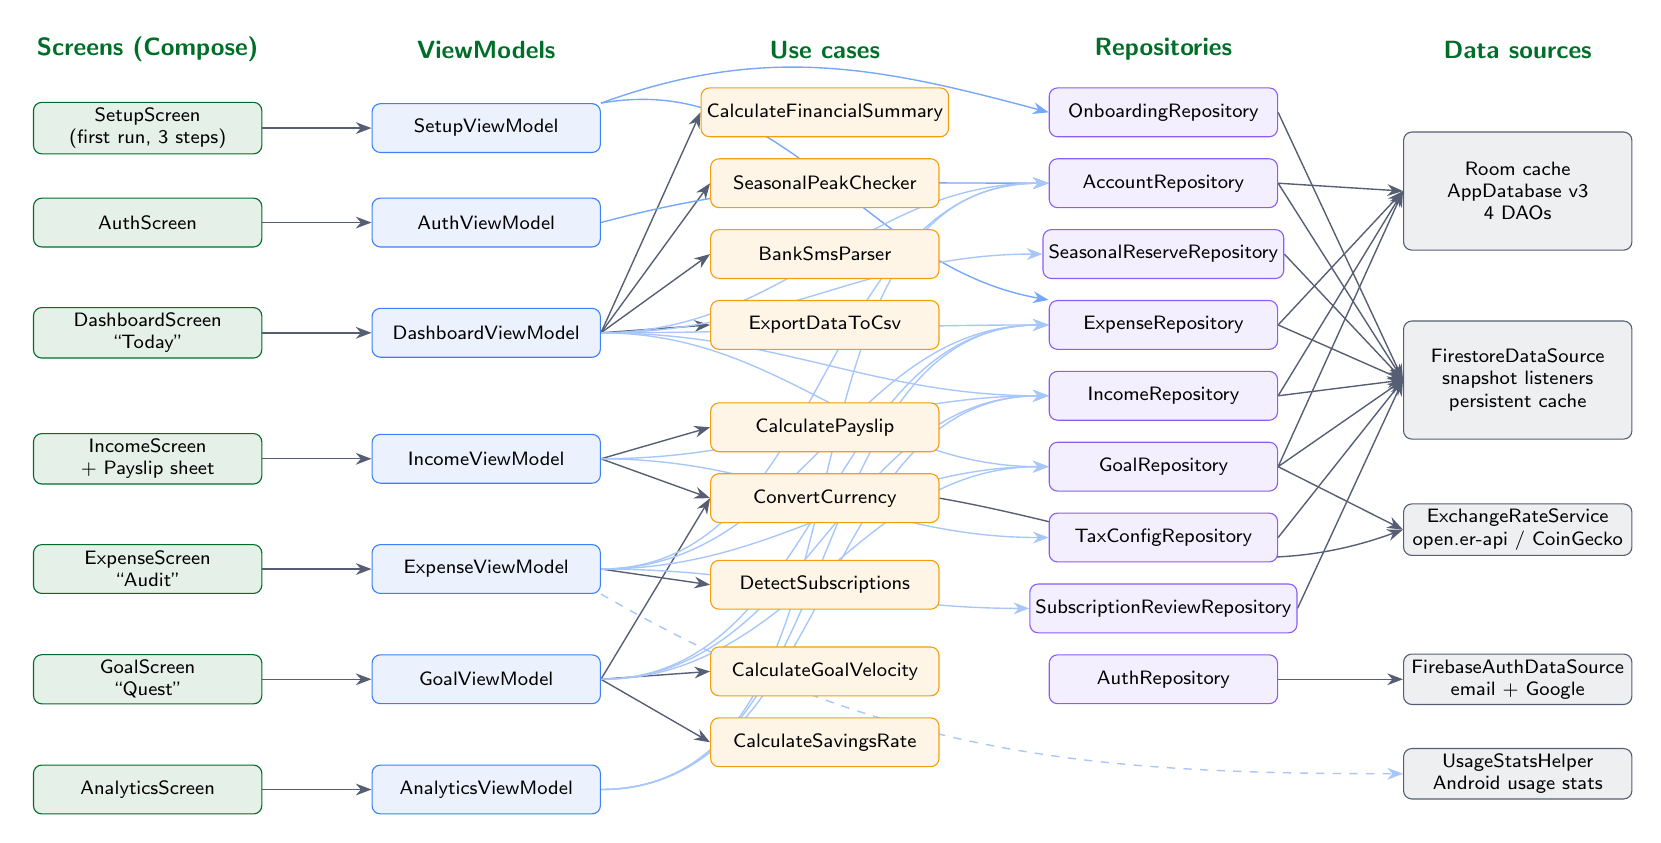
\begin{tikzpicture}[x=1cm,y=1cm]
% column titles
\foreach \x/\t in {0/Screens (Compose),4.3/ViewModels,8.6/Use cases,12.9/Repositories,17.4/Data sources}
  \node[font=\sffamily\bfseries\small,text=pfgreendark] at (\x,9.4) {\t};
% screens
\node[box=pfgreendark] (sSet)  at (0,8.4) {SetupScreen\\(first run, 3 steps)};
\node[box=pfgreendark] (sAuth) at (0,7.2) {AuthScreen};
\node[box=pfgreendark] (sDash) at (0,5.8) {DashboardScreen\\``Today''};
\node[box=pfgreendark] (sInc)  at (0,4.2) {IncomeScreen\\+ Payslip sheet};
\node[box=pfgreendark] (sExp)  at (0,2.8) {ExpenseScreen\\``Audit''};
\node[box=pfgreendark] (sGoal) at (0,1.4) {GoalScreen\\``Quest''};
\node[box=pfgreendark] (sAna)  at (0,0.0) {AnalyticsScreen};
% viewmodels
\node[box=pfblue] (vSet)  at (4.3,8.4) {SetupViewModel};
\node[box=pfblue] (vAuth) at (4.3,7.2) {AuthViewModel};
\node[box=pfblue] (vDash) at (4.3,5.8) {DashboardViewModel};
\node[box=pfblue] (vInc)  at (4.3,4.2) {IncomeViewModel};
\node[box=pfblue] (vExp)  at (4.3,2.8) {ExpenseViewModel};
\node[box=pfblue] (vGoal) at (4.3,1.4) {GoalViewModel};
\node[box=pfblue] (vAna)  at (4.3,0.0) {AnalyticsViewModel};
% use cases
\node[box=pfamber] (uSum)  at (8.6,8.6) {CalculateFinancialSummary};
\node[box=pfamber] (uSea)  at (8.6,7.7) {SeasonalPeakChecker};
\node[box=pfamber] (uSms)  at (8.6,6.8) {BankSmsParser};
\node[box=pfamber] (uCsv)  at (8.6,5.9) {ExportDataToCsv};
\node[box=pfamber] (uPay)  at (8.6,4.6) {CalculatePayslip};
\node[box=pfamber] (uFx)   at (8.6,3.7) {ConvertCurrency};
\node[box=pfamber] (uSub)  at (8.6,2.6) {DetectSubscriptions};
\node[box=pfamber] (uVel)  at (8.6,1.5) {CalculateGoalVelocity};
\node[box=pfamber] (uRate) at (8.6,0.6) {CalculateSavingsRate};
% repositories
\node[box=pfviolet] (rOnb)  at (12.9,8.6) {OnboardingRepository};
\node[box=pfviolet] (rAcc)  at (12.9,7.7) {AccountRepository};
\node[box=pfviolet] (rRes)  at (12.9,6.8) {SeasonalReserveRepository};
\node[box=pfviolet] (rExp)  at (12.9,5.9) {ExpenseRepository};
\node[box=pfviolet] (rInc)  at (12.9,5.0) {IncomeRepository};
\node[box=pfviolet] (rGoal) at (12.9,4.1) {GoalRepository};
\node[box=pfviolet] (rTax)  at (12.9,3.2) {TaxConfigRepository};
\node[box=pfviolet] (rSubR) at (12.9,2.3) {SubscriptionReviewRepository};
\node[box=pfviolet] (rAuth) at (12.9,1.4) {AuthRepository};
% data sources
\node[box=pfmuted,minimum height=1.5cm] (dRoom) at (17.4,7.6) {Room cache\\\code{AppDatabase} v3\\4 DAOs};
\node[box=pfmuted,minimum height=1.5cm] (dFs)   at (17.4,5.2) {\code{FirestoreDataSource}\\snapshot listeners\\persistent cache};
\node[box=pfmuted] (dRate) at (17.4,3.3) {\code{ExchangeRateService}\\open.er-api / CoinGecko};
\node[box=pfmuted] (dFa)   at (17.4,1.4) {\code{FirebaseAuthDataSource}\\email + Google};
\node[box=pfmuted] (dUse)  at (17.4,0.2) {\code{UsageStatsHelper}\\Android usage stats};
\begin{pgfonlayer}{background}
% screen -> vm
\foreach \s/\v in {sSet/vSet,sAuth/vAuth,sDash/vDash,sInc/vInc,sExp/vExp,sGoal/vGoal,sAna/vAna}
  \draw[arr] (\s) -- (\v);
% vm -> use cases
\foreach \u in {uSum,uSea,uSms,uCsv} \draw[arr] (vDash.east) -- (\u.west);
\foreach \u in {uPay,uFx} \draw[arr] (vInc.east) -- (\u.west);
\draw[arr] (vExp.east) -- (uSub.west);
\foreach \u in {uVel,uRate,uFx} \draw[arr] (vGoal.east) -- (\u.west);
% vm -> repositories (curved to keep them distinguishable)
\draw[arr,pfblue!70] (vSet.north east) to[out=20,in=165] (rOnb.west);
\draw[arr,pfblue!70] (vSet.north east) to[out=10,in=170] (rExp.north west);
\draw[arr,pfblue!70] (vAuth.east) to[out=15,in=180] (rAcc.west);
\foreach \r in {rAcc,rRes,rExp,rInc,rGoal} \draw[arr,pfblue!45] (vDash.east) to[out=0,in=180] (\r.west);
\foreach \r in {rInc,rTax} \draw[arr,pfblue!45] (vInc.east) to[out=0,in=180] (\r.west);
\foreach \r in {rExp,rGoal,rAcc,rSubR} \draw[arr,pfblue!45] (vExp.east) to[out=0,in=180] (\r.west);
\foreach \r in {rGoal,rInc,rExp} \draw[arr,pfblue!45] (vGoal.east) to[out=0,in=180] (\r.west);
\foreach \r in {rInc,rExp,rAcc} \draw[arr,pfblue!45] (vAna.east) to[out=0,in=180] (\r.west);
\draw[arr,pfblue!45,dashed] (vExp.south east) to[out=-30,in=180] (dUse.west);
% repositories -> sources
\foreach \r in {rAcc,rExp,rInc,rGoal} {\draw[arr] (\r.east) -- (dRoom.west); \draw[arr] (\r.east) -- (dFs.west);}
\foreach \r in {rOnb,rRes,rTax,rSubR} \draw[arr] (\r.east) -- (dFs.west);
\draw[arr] (rGoal.east) -- (dRate.west);
\draw[arr] (rAuth.east) -- (dFa.west);
\draw[arr] (uFx.east) to[out=-10,in=200] (dRate.west);
\end{pgfonlayer}
\end{tikzpicture}
\caption{MVVM diagram. Green: Compose screens; blue: ViewModels exposing \code{StateFlow}; amber: domain use cases; violet: repository interfaces (bound to implementations with Hilt \code{@Binds}); grey: data sources. The dashed arrow is a platform helper rather than a repository.}
\label{fig:mvvm}
\end{figure}
\end{landscape}

\subsection{How data flows}
\paragraph{Reads.} The account, expense, income and goal repositories return a \code{cacheBackedFlow}. The UI collects a Room \code{Flow}, so a screen shows cached data immediately with or without signal. While someone is collecting, a Firestore snapshot listener runs alongside it and writes every snapshot into Room with \code{replaceAll} in a transaction; Room then re-emits. When the screen goes away for more than five seconds (\code{WhileSubscribed(5000)}), the listener is removed. The goal repository also combines the goal with the day's USD rate, so a USD-linked target re-prices when a new rate arrives (\req{FR-GOAL-6}). Small per-user settings -- subscription decisions, seasonal reserves, the onboarding profile, and the tax bands -- rely on Firestore's own offline cache instead of Room.

\paragraph{Writes.} Figure~\ref{fig:write} shows Kavindu logging a coffee with no signal. Writes do not wait for the server: awaiting the Firestore task would hang until the device reconnects. Firestore's persistent queue, not an application flag, guarantees the upload.

\begin{figure}[H]
\centering
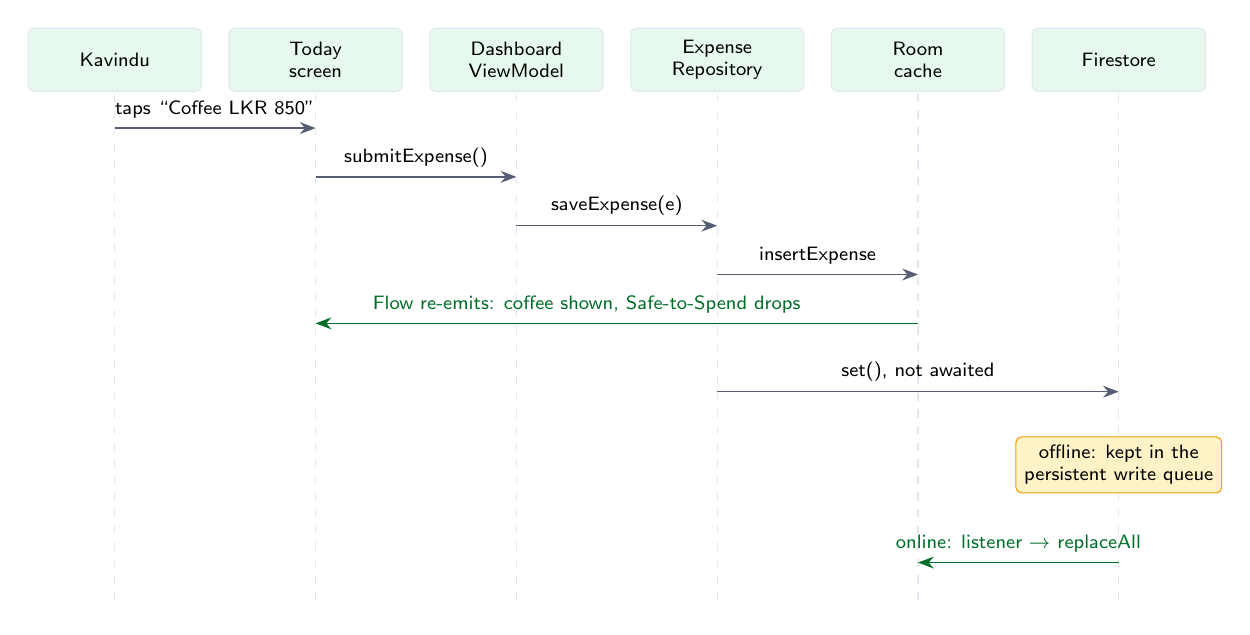
\begin{tikzpicture}[x=2.55cm,y=0.62cm,font=\sffamily\scriptsize]
\foreach \i/\n in {0/Kavindu,1/{Today\\screen},2/{Dashboard\\ViewModel},3/{Expense\\Repository},4/{Room\\cache},5/Firestore}{
  \node[draw=pfborder,fill=pfgreenlight,rounded corners=2pt,minimum width=2.2cm,minimum height=0.8cm,align=center] at (\i,0) {\n};
  \draw[pfborder,dashed] (\i,-0.7) -- (\i,-11.2);
}
\draw[arr] (0,-1.4) -- node[above]{taps ``Coffee \lkr{850}''} (1,-1.4);
\draw[arr] (1,-2.4) -- node[above]{\code{submitExpense()}} (2,-2.4);
\draw[arr] (2,-3.4) -- node[above]{\code{saveExpense(e)}} (3,-3.4);
\draw[arr] (3,-4.4) -- node[above]{\code{insertExpense}} (4,-4.4);
\draw[arr,pfgreendark] (4,-5.4) -- node[above,pos=0.55]{Flow re-emits: coffee shown, Safe-to-Spend drops} (1,-5.4);
\draw[arr] (3,-6.8) -- node[above]{\code{set()}, not awaited} (5,-6.8);
\node[fill=pfamberlight,draw=pfamber,rounded corners=2pt,align=center,inner sep=3pt] at (5,-8.3) {offline: kept in the\\persistent write queue};
\draw[arr,pfgreendark] (5,-10.3) -- node[above]{online: listener \textrightarrow{} \code{replaceAll}} (4,-10.3);
\end{tikzpicture}
\caption{Recording an expense offline. The coffee is visible instantly (\req{NFR-1}, \req{FR-EXP-6}) and uploads on reconnection (\req{NFR-3}).}
\label{fig:write}
\end{figure}

\subsection{Dependency injection and platform integrations}
Hilt provides the Room database and DAOs (\code{DatabaseModule}), Firebase Auth and Firestore with persistent cache settings (\code{FirebaseModule}), and binds every repository interface to its implementation (\code{RepositoryModule}). ViewModels are obtained with \code{hiltViewModel()} inside \code{AppNavGraph}; no ViewModel is created manually (C-7).

\begin{tabularx}{\textwidth}{@{}p{4.1cm}p{4cm}L@{}}
\toprule
\textbf{Feature} & \textbf{Where} & \textbf{Android mechanism}\\
\midrule
Share a bank SMS (\req{FR-EXP-7}) & \code{MainActivity}, \code{BankSmsParser} & Share sheet (\code{ACTION_SEND}, text/plain); no READ\_SMS\\
Reveal and copy account number (\req{FR-ACC-6}, \req{FR-ACC-7}) & \code{BiometricHelper} & \code{BiometricPrompt} (strong biometric or device credential); clipboard cleared after 60 s\\
Screens hidden from screenshots & \code{MainActivity} & \code{FLAG_SECURE}\\
App last opened (\req{FR-SUB-5}) & \code{UsageStatsHelper} & \code{UsageStatsManager} (special access)\\
CSV export (\req{FR-DATA-1}) & \code{ExportDataToCsvUseCase} & Share sheet (\code{ACTION_SEND}, text/csv)\\
Daily exchange rates (\req{FR-INC-5}) & \code{ExchangeRateService} & HTTPS on \code{Dispatchers.IO}, at most once a day (C-17)\\
\bottomrule
\end{tabularx}

% ============================================================================
\section{Firestore Schema}
\label{sec:schema}

\subsection{Collections}
Everything Kavindu records lives under his own user document, so a single rule protects it all (\req{NFR-5}) and the same data appears on any device he signs in on (\req{FR-AUTH-3}). App-wide configuration that is not his data lives in a separate read-only \code{config} collection.

\begin{lstlisting}
users/
  {uid}                                  user document
    subscriptionReviews : map            Keep / Cancel decisions             (FR-SUB-3, FR-SUB-4)
    seasonalReserves    : map            money set aside before a peak       (FR-LK-5)
    onboarding          : map            first-run setup answers             (FR-AUTH-4, FR-AUTH-5)
    accounts/{accountId}        AccountDto   where money is held or paid from  (P5)
    expenses/{expenseId}        ExpenseDto   money out                         (P5, P6, P7)
    income_streams/{incomeId}   IncomeDto    money in, received or invoiced    (P1-P4)
    goals/{goalId}              GoalDto      the MacBook goal                  (P8)

config/                                  read-only for signed-in users
  apitBands                     ApitConfigDto   APIT tax schedule              (FR-LK-2, C-16)
\end{lstlisting}

The three maps on the user document are small, are always read together with the user, and are written with \code{SetOptions.merge()} so that they never overwrite one another. Keeping them as maps rather than subcollections avoids three extra listeners per screen.

\subsection{Accounts}
Path: \code{users/{uid}/accounts/{accountId}}.

On first sign-in, \code{ensureDefaultAccounts} creates one zero-balance account per place Kavindu's money leaves from, so every expense can be attributed from the first entry. It checks the server first, so an empty offline cache is never mistaken for a new user.

\begin{tabularx}{\textwidth}{@{}p{4.1cm}p{1.7cm}p{3.2cm}L@{}}
\toprule
\textbf{Field} & \textbf{Type} & \textbf{Kavindu example} & \textbf{Why it exists}\\
\midrule
\code{id} & string & \code{acc_secondary_bank} & Fixed IDs for the four defaults\\
\code{name} & string & Secondary Account (Auto-Debits) & \\
\code{type} & string & \code{BANK_SECONDARY} & Primary, secondary, cash or crypto exchange (\req{FR-ACC-1})\\
\code{balanceLkr} & number & 0 & His own record, never imported (C-13)\\
\code{isAutoDebitSource} & boolean & true & Where the gym and forgotten subscriptions are charged (\prob{P6})\\
\code{accountNumber} & string & 1002938472 & Shown masked until biometric reveal (\req{FR-ACC-6})\\
\code{isFrozen}, \code{frozenUntilMillis} & boolean, number & false, null & Spending Freeze (\req{FR-ACC-3})\\
\code{freezeBreakCount} & number & 0 & Times he spent from a frozen account (\req{FR-ACC-5})\\
\bottomrule
\end{tabularx}

\subsection{Expenses}
Path: \code{users/{uid}/expenses/{expenseId}}.

\begin{tabularx}{\textwidth}{@{}p{4.1cm}p{1.7cm}p{3.2cm}L@{}}
\toprule
\textbf{Field} & \textbf{Type} & \textbf{Kavindu example} & \textbf{Why it exists}\\
\midrule
\code{title} & string & PickMe to office & Also the merchant key for subscription detection\\
\code{amountLkr} & number & 1450 & Always LKR\\
\code{category} & string & \code{TRANSPORT} & One of eight categories\\
\code{isCommitted} & boolean & false & Proposed from the category, flipped by him (\req{FR-EXP-2}, \prob{P7})\\
\code{paymentAccountId}, \code{paymentAccountName} & string & \code{acc_cash}, Cash in Hand & Covers cash and the secondary account (\req{FR-EXP-5}); name copied so lists render without a join\\
\code{timestamp}, \code{notes} & number, string & & \\
\bottomrule
\end{tabularx}

\subsection{Income}
Path: \code{users/{uid}/income_streams/{incomeId}}.

\begin{tabularx}{\textwidth}{@{}p{4.2cm}p{1.5cm}p{3.2cm}L@{}}
\toprule
\textbf{Field} & \textbf{Type} & \textbf{Kavindu example (AdSense)} & \textbf{Why it exists}\\
\midrule
\code{source} & string & \code{ADSENSE} & Salary, freelance, AdSense or crypto (\prob{P1})\\
\code{title}, \code{clientOrPlatform} & string & AdSense -- October; Google AdSense & For freelance, the client he invoices (\prob{P2})\\
\code{originalAmount} & number & 45 & In the original currency; negative for a crypto loss (\req{FR-INC-7})\\
\code{currency} & string & \code{USD} & LKR, USD, USDT or ETH\\
\code{exchangeRateToLkr} & number & 302.5 & \textbf{Frozen at save time} (ADR-0001); derived from what his bank credited (\req{FR-INC-6})\\
\code{amountInLkr} & number & 13612.5 & Stored, so October still matches his bank statement in March (\req{NFR-6})\\
\code{status} & string & \code{RECEIVED} & \code{RECEIVED} or \code{PENDING_INVOICE}; overdue is derived, never stored (\req{FR-INC-4})\\
\code{dateReceivedOrExpected} & number & & The due date while pending\\
\code{isRecurringMonthly} & boolean & false & True for his salary\\
\bottomrule
\end{tabularx}

\subsection{Savings goal}
Path: \code{users/{uid}/goals/{goalId}}.

\begin{tabularx}{\textwidth}{@{}p{4.2cm}p{1.5cm}p{3.2cm}L@{}}
\toprule
\textbf{Field} & \textbf{Type} & \textbf{Kavindu example} & \textbf{Why it exists}\\
\midrule
\code{title} & string & MacBook Pro M4 & \\
\code{targetAmountLkr} & number & 490000 & The target \emph{as he entered it}; never overwritten with the rate-adjusted value, so it cannot be scaled twice\\
\code{currentSavedLkr} & number & 11200 & Never changed by exchange-rate movements\\
\code{targetDateMillis}, \code{createdDateMillis} & number & 12 months out & Drives the required pace (\req{FR-GOAL-2})\\
\code{usdReferencePrice} & number or null & 1599 & Apple's USD price (\req{FR-GOAL-6})\\
\code{usdRateAtSetLkr}, \code{usdRateSetAtMillis} & number or null & 300.0 & Rate and time when the target was set\\
\bottomrule
\end{tabularx}

With a USD price, the app shows \(\text{target} \times \text{today's rate} \div \text{rate at set}\). If the rupee weakens from 300 to 306, his target becomes \lkr{499,800} and the goal card says ``Target + \lkr{9,800} since \ldots''.

\subsection{Maps on the user document}
\begin{lstlisting}
"subscriptionReviews": {
  "netflix_premium": { "decision": "CANCELLED", "decidedAt": 1730700000000, "consecutiveUnusedMonths": 0 },
  "gym_membership":  { "decision": "KEEP",      "decidedAt": 1730600000000, "consecutiveUnusedMonths": 2 }
},
"seasonalReserves": {
  "vesak_festival_2027": { "amountLkr": 20000, "setAsideAt": 1776000000000, "peakDateMillis": 1778800000000 }
},
"onboarding": {
  "monthlySalaryLkr": 126400,
  "incomeSources": { "SALARY": "LOW", "FREELANCE": "MODERATE", "ADSENSE": "MODERATE", "CRYPTO": "VOLATILE" },
  "fixedCommitments": [ { "title": "Rent", "amountLkr": 34000, "category": "RENT" },
                        { "title": "Fiber Broadband", "amountLkr": 4800, "category": "UTILITIES" } ],
  "completedAt": 1730750000000,
  "runwayMonths": 3,
  "runwaySavedLkr": 11200
}
\end{lstlisting}
\begin{itemize}
  \item \textbf{Subscription keys} are the merchant title lower-cased with non-alphanumerics replaced by underscores. A charge after \code{CANCELLED} marks the subscription ``still charging''; two consecutive ``didn't use it'' answers make its risk High (\req{FR-SUB-3}, \req{FR-SUB-4}).
  \item \textbf{A seasonal reserve is an earmark, not a transaction.} It lowers Safe-to-Spend only in the month it was set aside and until the peak day; after that the festival spending itself is recorded, so keeping the reserve would count the money twice (\req{FR-LK-5}).
  \item \textbf{Onboarding} records his salary, each active source with its variability and his fixed commitments (\req{FR-AUTH-4}, \req{FR-AUTH-5}).
\end{itemize}

\subsection{Configuration: APIT tax bands}
Path: \code{config/apitBands}.

\begin{lstlisting}
{ "effectiveFrom": "2025-04-01",
  "bands": [ { "lowerLkr": 0,      "upperLkr": 100000, "rate": 0.00 },
             { "lowerLkr": 100000, "upperLkr": 141667, "rate": 0.06 },
             { "lowerLkr": 141667, "upperLkr": 183333, "rate": 0.12 },
             { "lowerLkr": 183333, "upperLkr": 225000, "rate": 0.18 },
             { "lowerLkr": 225000, "upperLkr": 266667, "rate": 0.24 },
             { "lowerLkr": 266667, "upperLkr": 308333, "rate": 0.30 },
             { "lowerLkr": 308333, "upperLkr": null,   "rate": 0.36 } ] }
\end{lstlisting}
The payslip calculator validates the schedule (starts at 0, contiguous, rates between 0 and 1) and falls back to the bands bundled in the app if the document is missing or invalid. For a gross salary of \lkr{140,000} this gives APIT of \lkr{2,400} and employee EPF of \lkr{11,200}, leaving a take-home of \lkr{126,400} -- the figure Kavindu could not recall from his payslip (\prob{P10}).

\subsection{Security rules}
\begin{lstlisting}
rules_version = '2';
service cloud.firestore {
  match /databases/{database}/documents {
    match /users/{userId} {
      allow read, write: if request.auth != null && request.auth.uid == userId;
      match /accounts/{accountId} {
        allow read, write: if request.auth != null && request.auth.uid == userId;
      }
      match /income_streams/{incomeId} {
        allow read, write: if request.auth != null && request.auth.uid == userId;
      }
      match /expenses/{expenseId} {
        allow read, write: if request.auth != null && request.auth.uid == userId;
      }
      match /goals/{goalId} {
        allow read, write: if request.auth != null && request.auth.uid == userId;
      }
    }
    match /config/{docId} {
      allow read: if request.auth != null;
      allow write: if false;
    }
  }
}
\end{lstlisting}
Unauthenticated requests are refused; another signed-in user can never read Kavindu's documents; configuration is read-only from the app; every other path is denied by default.

\subsection{Local cache and entity-relationship model}
Room (\code{AppDatabase}, version 3) mirrors the four collections in the tables \code{accounts}, \code{expenses}, \code{income_streams} and \code{savings_goals}. It is only a cache: it uses \code{fallbackToDestructiveMigration()}, and pending offline writes are not lost when it is rebuilt because they are queued in Firestore's own cache.

\begin{figure}[H]
\centering
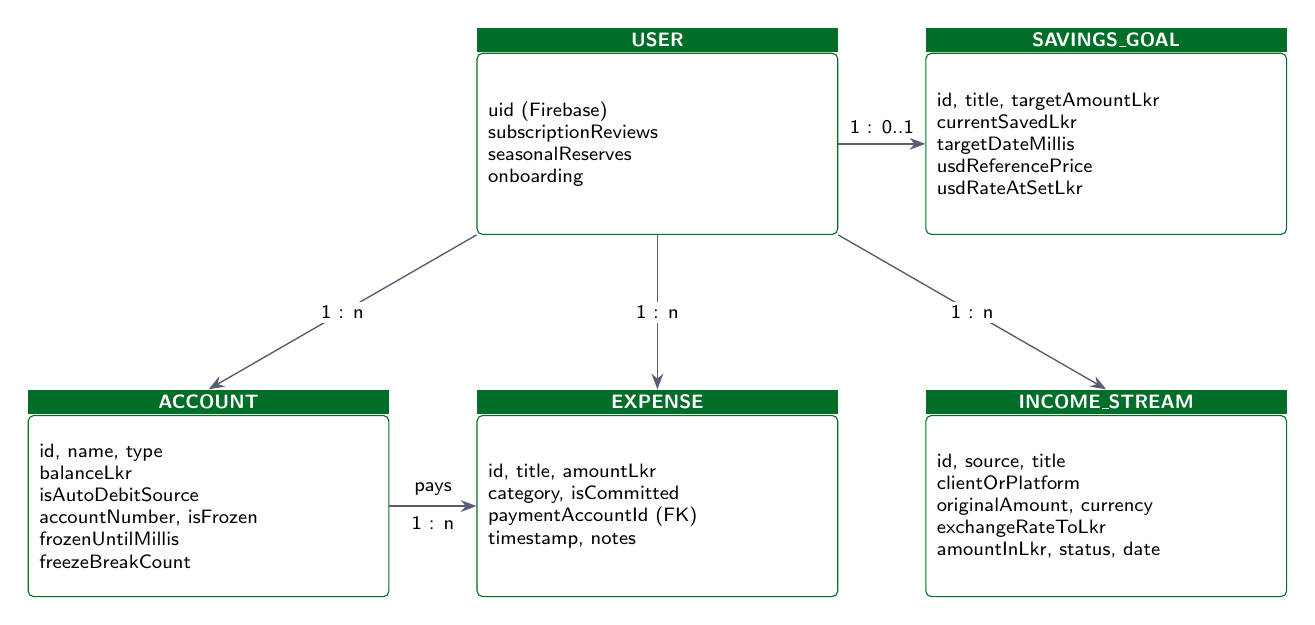
\begin{tikzpicture}[font=\sffamily\scriptsize,
  ent/.style={draw=pfgreendark,fill=white,rounded corners=2pt,align=left,inner sep=4pt,text width=4.3cm,minimum height=2.3cm,anchor=north},
  head/.style={fill=pfgreendark,text=white,font=\sffamily\bfseries\scriptsize,minimum width=4.3cm+8pt,inner sep=2pt,anchor=south},
  lab/.style={fill=white,inner sep=1.5pt,font=\sffamily\scriptsize}]
\node[ent] (user) at (0,0) {\code{uid} (Firebase)\\subscriptionReviews\\seasonalReserves\\onboarding};
\node[head] (userH) at (user.north) {USER};
\node[ent] (acc) at (-5.7,-4.6) {\code{id}, name, type\\balanceLkr\\isAutoDebitSource\\accountNumber, isFrozen\\frozenUntilMillis\\freezeBreakCount};
\node[head] (accH) at (acc.north) {ACCOUNT};
\node[ent] (exp) at (0,-4.6) {\code{id}, title, amountLkr\\category, isCommitted\\paymentAccountId (FK)\\timestamp, notes};
\node[head] (expH) at (exp.north) {EXPENSE};
\node[ent] (inc) at (5.7,-4.6) {\code{id}, source, title\\clientOrPlatform\\originalAmount, currency\\exchangeRateToLkr\\amountInLkr, status, date};
\node[head] (incH) at (inc.north) {INCOME\_STREAM};
\node[ent] (goal) at (5.7,0) {\code{id}, title, targetAmountLkr\\currentSavedLkr\\targetDateMillis\\usdReferencePrice\\usdRateAtSetLkr};
\node[head] (goalH) at (goal.north) {SAVINGS\_GOAL};
\draw[arr] (user.south west) -- node[lab,pos=0.5]{1 : n} (accH.north);
\draw[arr] (user.south) -- node[lab,pos=0.5]{1 : n} (expH.north);
\draw[arr] (user.south east) -- node[lab,pos=0.5]{1 : n} (incH.north);
\draw[arr] (user.east) -- node[lab,above=2pt]{1 : 0..1} (goal.west);
\draw[arr] (acc.east) -- node[lab,above=2pt]{pays} node[lab,below=2pt]{1 : n} (exp.west);
\end{tikzpicture}
\caption{Entity-relationship model. The three maps are fields of the user document; the app reads one goal per user (the earliest created).}
\end{figure}

% ============================================================================
\section{Annotated Wireframes}
\label{sec:wireframes}
The wireframes below show each main screen as built, with the layout, labels and order of elements taken from the Compose code. Each numbered callout is explained in the table beside it: what the element does for Kavindu and which problem and requirement it serves. The bottom dock (Today, Analytics, Income, Quest, Audit) is the same on every screen after setup. Amounts and names in the wireframes are illustrative values drawn from Kavindu's scenario, not data from a real account.

% ---- Setup ----------------------------------------------------------------
\subsection{First-run setup}
\begin{minipage}[t]{0.42\textwidth}\vspace{0pt}
\centering
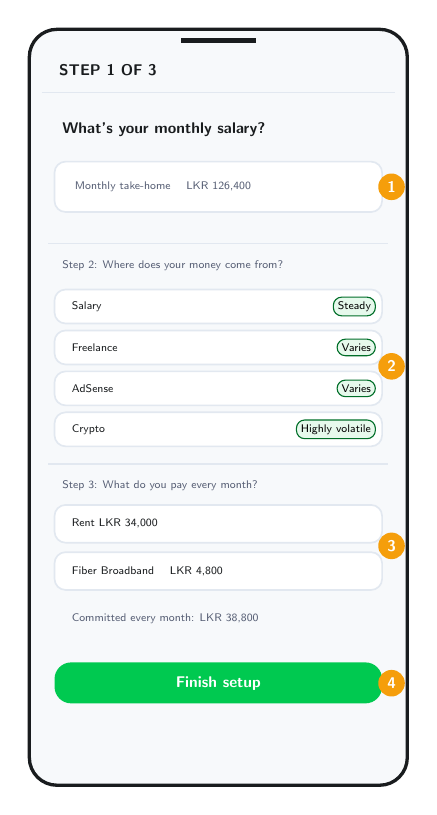
\begin{tikzpicture}[scale=0.8,every node/.style={scale=0.8}]
\phoneframe{STEP 1 OF 3}
\node[wftext,font=\sffamily\scriptsize\bfseries] at (0.4,10.4) {What's your monthly salary?};
\draw[card] (0.4,9.1) rectangle (5.6,9.9); \node[wfmuted] at (0.6,9.5) {Monthly take-home \quad LKR 126,400};
\node[num] at (5.75,9.5) {1};
\draw[pfborder] (0.3,8.6) -- (5.7,8.6);
\node[wfmuted] at (0.4,8.25) {Step 2: Where does your money come from?};
\foreach \y/\s/\v in {7.6/Salary/Steady,6.95/Freelance/Varies,6.3/AdSense/Varies,5.65/Crypto/Highly volatile}{
  \draw[card] (0.4,\y-0.27) rectangle (5.6,\y+0.27);
  \node[wftext] at (0.55,\y) {\s};
  \node[chipon,anchor=east] at (5.5,\y) {\v};
}
\node[num] at (5.75,6.65) {2};
\draw[pfborder] (0.3,5.1) -- (5.7,5.1);
\node[wfmuted] at (0.4,4.75) {Step 3: What do you pay every month?};
\draw[card] (0.4,3.85) rectangle (5.6,4.45); \node[wftext] at (0.55,4.15) {Rent \hfill LKR 34,000};
\draw[card] (0.4,3.1) rectangle (5.6,3.7);  \node[wftext] at (0.55,3.4) {Fiber Broadband \quad LKR 4,800};
\node[wfmuted] at (0.55,2.65) {Committed every month: LKR 38,800};
\node[num] at (5.75,3.8) {3};
\fill[pfgreen,rounded corners=6pt] (0.4,1.3) rectangle (5.6,1.95);
\node[text=white,font=\sffamily\scriptsize\bfseries] at (3,1.62) {Finish setup};
\node[num] at (5.75,1.62) {4};
\end{tikzpicture}
\end{minipage}\hfill
\begin{minipage}[t]{0.55\textwidth}\vspace{0pt}
\small
\begin{tabularx}{\linewidth}{@{}p{0.45cm}L@{}}
\toprule
\# & \textbf{Element and justification}\\
\midrule
\callout{1} & \textbf{Monthly take-home.} Optional, because not every user has a salary. Gives the dashboard an Income Basis before his first payslip is logged. \prob{P1}, \req{FR-AUTH-4}\\
\callout{2} & \textbf{Sources with variability.} Each active source is ticked and given steady / varies / highly volatile, pre-filled sensibly (crypto starts as volatile). Volatile sources are treated more cautiously. \prob{P1}, \prob{P4}, \req{FR-AUTH-5}\\
\callout{3} & \textbf{Fixed commitments.} Rent \lkr{34,000} is suggested because it is in his scenario; the running total shows what is committed before he spends anything. Below it he picks a safety buffer of 1--6 months of those costs (three is preselected), which the dashboard later tracks. \prob{P7}, \req{FR-AUTH-4}, \req{FR-AUTH-6}\\
\callout{4} & \textbf{Three short steps, one screen each.} His Google Sheet died of entry overhead (F1), so setup asks only what the dashboard needs on day one. Written once to \code{users/{uid}.onboarding}.\\
\bottomrule
\end{tabularx}
\end{minipage}

% ---- Dashboard --------------------------------------------------------------
\subsection{Today (dashboard)}
\begin{minipage}[t]{0.42\textwidth}\vspace{0pt}
\centering
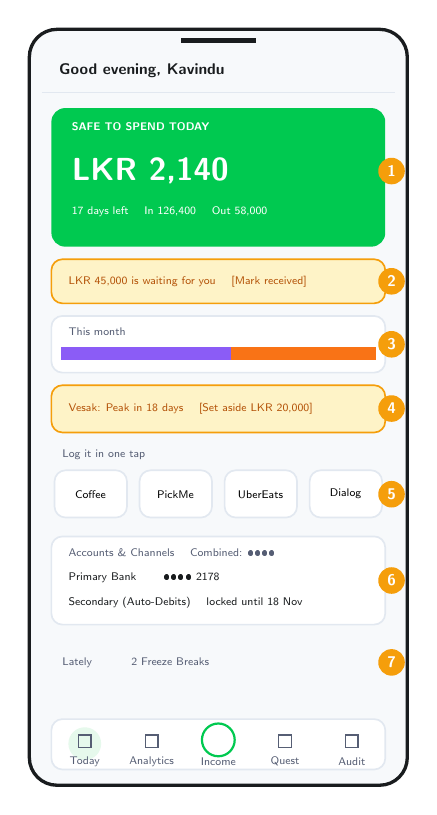
\begin{tikzpicture}[scale=0.8,every node/.style={scale=0.8}]
\phoneframe{Good evening, Kavindu}
\fill[hero] (0.35,8.55) rectangle (5.65,10.75);
\node[text=white,font=\sffamily\tiny\bfseries,anchor=west] at (0.55,10.45) {SAFE TO SPEND TODAY};
\node[text=white,font=\sffamily\Large\bfseries,anchor=west] at (0.55,9.75) {LKR 2,140};
\node[text=white,font=\sffamily\tiny,anchor=west] at (0.55,9.1) {17 days left \quad In 126,400 \quad Out 58,000};
\node[num] at (5.75,9.75) {1};
\draw[warn] (0.35,7.65) rectangle (5.65,8.35);
\node[wftext,text=pfamberdark] at (0.5,8.0) {LKR 45,000 is waiting for you \quad [Mark received]};
\node[num] at (5.75,8.0) {2};
\draw[card] (0.35,6.55) rectangle (5.65,7.45);
\node[wfmuted] at (0.5,7.2) {This month};
\fill[pfviolet] (0.5,6.75) rectangle (3.2,6.95); \fill[pforange] (3.2,6.75) rectangle (5.5,6.95);
\node[num] at (5.75,7.0) {3};
\draw[warn] (0.35,5.6) rectangle (5.65,6.35);
\node[wftext,text=pfamberdark] at (0.5,5.98) {Vesak: Peak in 18 days \quad [Set aside LKR 20,000]};
\node[num] at (5.75,5.98) {4};
\node[wfmuted] at (0.4,5.25) {Log it in one tap};
\foreach \x/\t in {0.4/Coffee,1.75/PickMe,3.1/UberEats,4.45/Dialog}{
  \draw[card] (\x,4.25) rectangle (\x+1.15,5.0); \node[font=\sffamily\tiny] at (\x+0.57,4.62) {\t};}
\node[num] at (5.75,4.62) {5};
\draw[card] (0.35,2.55) rectangle (5.65,3.95);
\node[wfmuted] at (0.5,3.7) {Accounts \& Channels \quad Combined: \textbullet\textbullet\textbullet\textbullet};
\node[wftext] at (0.5,3.3) {Primary Bank \quad\quad \textbullet\textbullet\textbullet\textbullet{} 2178};
\node[wftext] at (0.5,2.9) {Secondary (Auto-Debits) \quad locked until 18 Nov};
\node[num] at (5.75,3.25) {6};
\node[wfmuted] at (0.4,1.95) {Lately \quad\quad\quad 2 Freeze Breaks};
\node[num] at (5.75,1.95) {7};
\dock{1}
\end{tikzpicture}
\end{minipage}\hfill
\begin{minipage}[t]{0.55\textwidth}\vspace{0pt}
\small
\begin{tabularx}{\linewidth}{@{}p{0.45cm}L@{}}
\toprule
\# & \textbf{Element and justification}\\
\midrule
\callout{1} & \textbf{Safe to spend today.} One number he can act on at the till: (Income Basis $-$ committed $-$ goal saving $-$ discretionary so far) $\div$ days left. Monthly in/out sits underneath as context, not the headline. \prob{P1}, \prob{P7}, \req{FR-DASH-1}--\req{FR-DASH-3}\\
\callout{2} & \textbf{Overdue invoice, amber not red.} Names the client and amount, with one-tap ``Mark received''. Unpaid invoices are never part of the allowance. \prob{P2}, \req{FR-DASH-2}, \req{FR-DASH-5}\\
\callout{3} & \textbf{Committed vs discretionary bar} with amounts: rent and broadband against coffee, PickMe and UberEats. \prob{P7}, \req{FR-DASH-4}\\
\callout{4} & \textbf{Seasonal Peak warning} 30 days ahead, with last year's excess if known and a one-tap ``Set aside'' that holds the amount back from Safe-to-Spend. \prob{P11}, \req{FR-LK-4}, \req{FR-LK-5}\\
\callout{5} & \textbf{One-tap presets} from his own most repeated spends, topped up with Sri Lankan starters. Three taps, five seconds. \prob{P9}, \req{FR-EXP-3}, \req{NFR-1}\\
\callout{6} & \textbf{Accounts.} Masked numbers revealed by fingerprint; a frozen account shows as locked. \prob{P5}, \req{FR-ACC-2}, \req{FR-ACC-3}, \req{FR-ACC-6}\\
\callout{7} & \textbf{Freeze Breaks} counted without blame; spending is never refused. \req{FR-ACC-4}, \req{FR-ACC-5}\\
\bottomrule
\end{tabularx}
\end{minipage}

% ---- Income -----------------------------------------------------------------
\subsection{Income hub}
\begin{minipage}[t]{0.42\textwidth}\vspace{0pt}
\centering
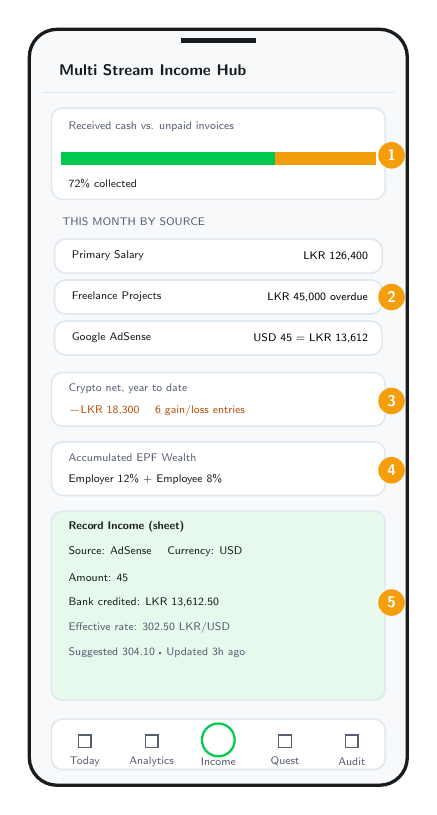
\begin{tikzpicture}[scale=0.8,every node/.style={scale=0.8}]
\phoneframe{Multi Stream Income Hub}
\draw[card] (0.35,9.3) rectangle (5.65,10.75);
\node[wfmuted] at (0.5,10.45) {Received cash vs. unpaid invoices};
\fill[pfgreen] (0.5,9.85) rectangle (3.9,10.05); \fill[pfamber] (3.9,9.85) rectangle (5.5,10.05);
\node[wftext] at (0.5,9.55) {72\% collected};
\node[num] at (5.75,10.0) {1};
\node[wfmuted] at (0.4,8.95) {THIS MONTH BY SOURCE};
\foreach \y/\s/\a in {8.4/Primary Salary/{LKR 126,400},7.75/Freelance Projects/{LKR 45,000 overdue},7.1/Google AdSense/{USD 45 = LKR 13,612}}{
  \draw[card] (0.4,\y-0.27) rectangle (5.6,\y+0.27);
  \node[wftext] at (0.55,\y) {\s}; \node[font=\sffamily\tiny,anchor=east] at (5.5,\y) {\a};}
\node[num] at (5.75,7.75) {2};
\draw[card] (0.35,5.7) rectangle (5.65,6.55);
\node[wfmuted] at (0.5,6.3) {Crypto net, year to date};
\node[wftext,text=pfamberdark] at (0.5,5.95) {$-$LKR 18,300 \quad 6 gain/loss entries};
\node[num] at (5.75,6.1) {3};
\draw[card] (0.35,4.6) rectangle (5.65,5.45);
\node[wfmuted] at (0.5,5.2) {Accumulated EPF Wealth};
\node[wftext] at (0.5,4.85) {Employer 12\% + Employee 8\%};
\node[num] at (5.75,5.0) {4};
\draw[card,fill=pfgreenlight] (0.35,1.35) rectangle (5.65,4.35);
\node[wftext,font=\sffamily\tiny\bfseries] at (0.5,4.1) {Record Income (sheet)};
\node[wftext] at (0.5,3.7) {Source: AdSense \quad Currency: USD};
\node[wftext] at (0.5,3.3) {Amount: 45};
\node[wftext] at (0.5,2.9) {Bank credited: LKR 13,612.50};
\node[wfmuted] at (0.5,2.5) {Effective rate: 302.50 LKR/USD};
\node[wfmuted] at (0.5,2.1) {Suggested 304.10 \textperiodcentered{} Updated 3h ago};
\node[num] at (5.75,2.9) {5};
\dock{3}
\end{tikzpicture}
\end{minipage}\hfill
\begin{minipage}[t]{0.55\textwidth}\vspace{0pt}
\small
\begin{tabularx}{\linewidth}{@{}p{0.45cm}L@{}}
\toprule
\# & \textbf{Element and justification}\\
\midrule
\callout{1} & \textbf{Received vs unpaid.} The first honest answer to ``what did I earn this month?'' -- realised money in green, invoices still owed in amber. \prob{P1}, \req{FR-INC-9}\\
\callout{2} & \textbf{By source}, each in its own currency next to its LKR value. The freelance milestone turns overdue on its own once the due date passes. \prob{P2}, \req{FR-INC-1}, \req{FR-INC-4}, \req{FR-LK-6}\\
\callout{3} & \textbf{Crypto net, year to date.} Losses are negative income, so the Q1 gain and Q3 loss net out honestly. \prob{P4}, \req{FR-INC-7}, \req{FR-INC-8}\\
\callout{4} & \textbf{EPF balance} shown as savings he already owns; the payslip sheet derives EPF and APIT from gross salary using the bands in Firestore. \prob{P10}, \req{FR-LK-1}--\req{FR-LK-3}\\
\callout{5} & \textbf{What the bank actually credited.} The fetched rate is only a suggestion with its age; he types the LKR that arrived and the effective rate is stored and frozen. This is why past months still match his bank (ADR-0001). \prob{P3}, \req{FR-INC-2}, \req{FR-INC-5}, \req{FR-INC-6}\\
\bottomrule
\end{tabularx}
\end{minipage}

% ---- Audit ------------------------------------------------------------------
\subsection{Audit (expenses and subscriptions)}
\begin{minipage}[t]{0.42\textwidth}\vspace{0pt}
\centering
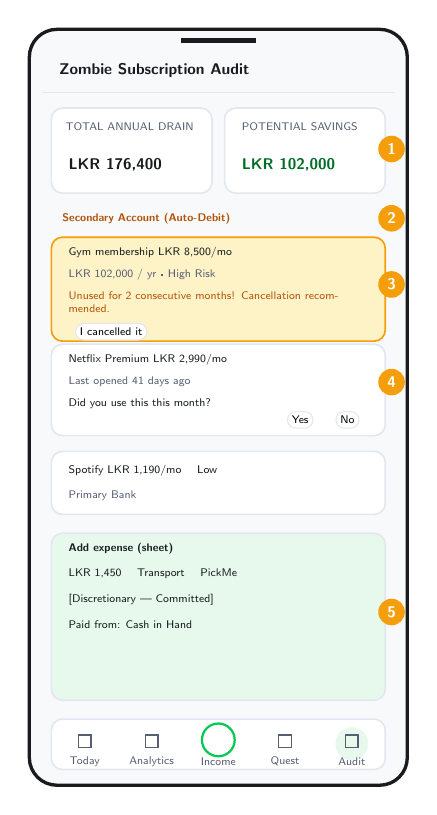
\begin{tikzpicture}[scale=0.8,every node/.style={scale=0.8}]
\phoneframe{Zombie Subscription Audit}
\draw[card] (0.35,9.4) rectangle (2.9,10.75); \draw[card] (3.1,9.4) rectangle (5.65,10.75);
\node[wfmuted] at (0.45,10.45) {TOTAL ANNUAL DRAIN}; \node[wftext,font=\sffamily\scriptsize\bfseries] at (0.5,9.85) {LKR 176,400};
\node[wfmuted] at (3.25,10.45) {POTENTIAL SAVINGS};  \node[wftext,font=\sffamily\scriptsize\bfseries,text=pfgreendark] at (3.25,9.85) {LKR 102,000};
\node[num] at (5.75,10.1) {1};
\node[wftext,font=\sffamily\tiny\bfseries,text=pfamberdark] at (0.4,9.0) {Secondary Account (Auto-Debit)};
\node[num] at (5.75,9.0) {2};
\draw[warn] (0.35,7.05) rectangle (5.65,8.7);
\node[wftext] at (0.5,8.45) {Gym membership \hfill LKR 8,500/mo};
\node[wfmuted] at (0.5,8.1) {LKR 102,000 / yr \textperiodcentered{} High Risk};
\node[wftext,text=pfamberdark,text width=4.7cm] at (0.5,7.67) {Unused for 2 consecutive months! Cancellation recommended.};
\node[chip] at (1.3,7.2) {I cancelled it};
\node[num] at (5.75,7.95) {3};
\draw[card] (0.35,5.55) rectangle (5.65,7.0);
\node[wftext] at (0.5,6.75) {Netflix Premium \hfill LKR 2,990/mo};
\node[wfmuted] at (0.5,6.4) {Last opened 41 days ago};
\node[wftext] at (0.5,6.05) {Did you use this this month?};
\node[chip] at (4.3,5.8) {Yes}; \node[chip] at (5.05,5.8) {No};
\node[num] at (5.75,6.4) {4};
\draw[card] (0.35,4.3) rectangle (5.65,5.3);
\node[wftext] at (0.5,5.0) {Spotify \hfill LKR 1,190/mo \quad Low};
\node[wfmuted] at (0.5,4.6) {Primary Bank};
\draw[card,fill=pfgreenlight] (0.35,1.35) rectangle (5.65,4.0);
\node[wftext,font=\sffamily\tiny\bfseries] at (0.5,3.75) {Add expense (sheet)};
\node[wftext] at (0.5,3.35) {LKR 1,450 \quad Transport \quad PickMe};
\node[wftext] at (0.5,2.95) {[Discretionary | Committed]};
\node[wftext] at (0.5,2.55) {Paid from: Cash in Hand};
\node[num] at (5.75,2.75) {5};
\dock{5}
\end{tikzpicture}
\end{minipage}\hfill
\begin{minipage}[t]{0.55\textwidth}\vspace{0pt}
\small
\begin{tabularx}{\linewidth}{@{}p{0.45cm}L@{}}
\toprule
\# & \textbf{Element and justification}\\
\midrule
\callout{1} & \textbf{Annual drain and potential savings.} A monthly LKR 8,500 is easy to ignore; LKR 102,000 a year is not. \prob{P6}, \req{FR-SUB-2}\\
\callout{2} & \textbf{Grouped by account, secondary first.} His bank app never showed the auto-debit account; this group is where the forgotten charges live. \prob{P5}, \prob{P6}, \req{FR-SUB-6}\\
\callout{3} & \textbf{Risk with a reason.} High after two ``No'' answers, after 30+ days unopened, or when still charging after a cancel. ``I cancelled it'' records the decision so a later charge is caught. \req{FR-SUB-3}, \req{FR-SUB-4}\\
\callout{4} & \textbf{One question after each charge.} ``Did you use this this month?'' replaces any automatic guess; app-usage data adds evidence when usage access is granted. \req{FR-SUB-4}, \req{FR-SUB-5}\\
\callout{5} & \textbf{Add expense.} The category proposes discretionary or committed and he flips it in one tap; any account, including cash. This is what fixed ``PickMe filed as online retail''. \prob{P5}, \prob{P7}, \req{FR-EXP-1}, \req{FR-EXP-2}, \req{FR-EXP-5}\\
\bottomrule
\end{tabularx}
\end{minipage}

% ---- Quest ------------------------------------------------------------------
\subsection{Quest (savings goal)}
\begin{minipage}[t]{0.42\textwidth}\vspace{0pt}
\centering
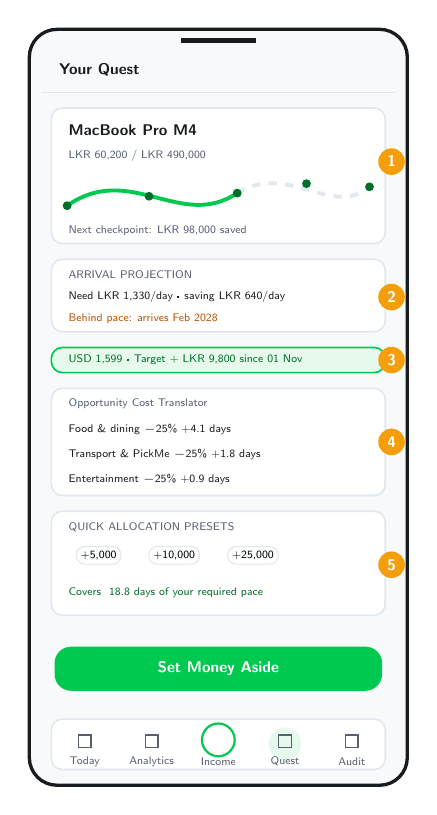
\begin{tikzpicture}[scale=0.8,every node/.style={scale=0.8}]
\phoneframe{Your Quest}
\draw[card] (0.35,8.6) rectangle (5.65,10.75);
\node[wftext,font=\sffamily\scriptsize\bfseries] at (0.5,10.4) {MacBook Pro M4};
\node[wfmuted] at (0.5,10.0) {LKR 60,200 / LKR 490,000};
\draw[pfgreen,line width=1.4pt] (0.6,9.2) .. controls (1.6,9.9) and (2.4,8.8) .. (3.3,9.4);
\draw[pfborder,line width=1.4pt,dashed] (3.3,9.4) .. controls (4.1,9.9) and (4.8,9.0) .. (5.4,9.5);
\foreach \x/\y in {0.6/9.2,1.9/9.35,3.3/9.4,4.4/9.55,5.4/9.5} \fill[pfgreendark] (\x,\y) circle (0.07);
\node[wfmuted] at (0.5,8.8) {Next checkpoint: LKR 98,000 saved};
\node[num] at (5.75,9.9) {1};
\draw[card] (0.35,7.2) rectangle (5.65,8.35);
\node[wfmuted] at (0.5,8.1) {ARRIVAL PROJECTION};
\node[wftext] at (0.5,7.75) {Need LKR 1,330/day \textperiodcentered{} saving LKR 640/day};
\node[wftext,text=pfamberdark] at (0.5,7.4) {Behind pace: arrives Feb 2028};
\node[num] at (5.75,7.75) {2};
\draw[warn,fill=pfgreenlight,draw=pfgreen] (0.35,6.55) rectangle (5.65,6.95);
\node[wftext,text=pfgreendark] at (0.5,6.75) {USD 1,599 \textperiodcentered{} Target + LKR 9,800 since 01 Nov};
\node[num] at (5.75,6.75) {3};
\draw[card] (0.35,4.6) rectangle (5.65,6.3);
\node[wfmuted] at (0.5,6.05) {Opportunity Cost Translator};
\node[wftext] at (0.5,5.65) {Food \& dining $-$25\% \hfill +4.1 days};
\node[wftext] at (0.5,5.25) {Transport \& PickMe $-$25\% \hfill +1.8 days};
\node[wftext] at (0.5,4.85) {Entertainment $-$25\% \hfill +0.9 days};
\node[num] at (5.75,5.45) {4};
\draw[card] (0.35,2.7) rectangle (5.65,4.35);
\node[wfmuted] at (0.5,4.1) {QUICK ALLOCATION PRESETS};
\node[chip] at (1.1,3.65) {+5,000}; \node[chip] at (2.3,3.65) {+10,000}; \node[chip] at (3.55,3.65) {+25,000};
\node[wftext,text=pfgreendark] at (0.5,3.05) {Covers ~18.8 days of your required pace};
\node[num] at (5.75,3.5) {5};
\fill[pfgreen,rounded corners=6pt] (0.4,1.5) rectangle (5.6,2.2);
\node[text=white,font=\sffamily\scriptsize\bfseries] at (3,1.85) {Set Money Aside};
\dock{4}
\end{tikzpicture}
\end{minipage}\hfill
\begin{minipage}[t]{0.55\textwidth}\vspace{0pt}
\small
\begin{tabularx}{\linewidth}{@{}p{0.45cm}L@{}}
\toprule
\# & \textbf{Element and justification}\\
\midrule
\callout{1} & \textbf{The goal as a journey of ten real-rupee levels} (\lkr{49,000} each). Progress only moves forward: no streaks or lives to lose, because a gap in tracking ended his Google Sheet. \prob{P9}, \req{NFR-2}\\
\callout{2} & \textbf{Required vs actual pace.} \lkr{478,800} left over 12 months is about \lkr{1,330} a day; his actual savings rate comes from what he recorded over the last 90 days. The arrival date says whether he is on pace and by how much. \prob{P8}, \req{FR-GOAL-2}--\req{FR-GOAL-4}\\
\callout{3} & \textbf{USD-linked target.} Apple prices in dollars; when the rupee moves, the reseller target moves with it, and the change is shown rather than hidden. \req{FR-GOAL-6}\\
\callout{4} & \textbf{Opportunity Cost Translator.} His top three discretionary categories from the last 30 days, each trimmed by a quarter, priced in days of MacBook. \prob{P11}, \req{FR-GOAL-5}\\
\callout{5} & \textbf{Windfall boosters} for a freelance milestone, with immediate feedback in days. \req{FR-GOAL-7}\\
\bottomrule
\end{tabularx}
\end{minipage}

% ---- Analytics --------------------------------------------------------------
\subsection{Analytics}
\begin{minipage}[t]{0.42\textwidth}\vspace{0pt}
\centering
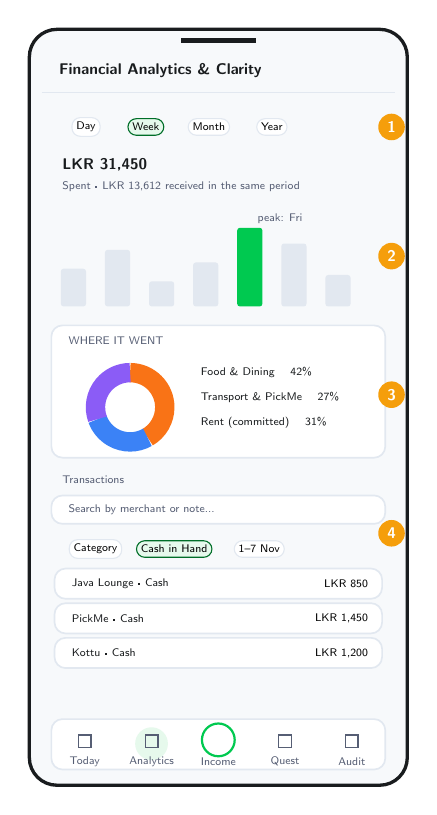
\begin{tikzpicture}[scale=0.8,every node/.style={scale=0.8}]
\phoneframe{Financial Analytics \& Clarity}
\node[chip] at (0.9,10.45) {Day}; \node[chipon] at (1.85,10.45) {Week}; \node[chip] at (2.85,10.45) {Month}; \node[chip] at (3.85,10.45) {Year};
\node[num] at (5.75,10.45) {1};
\node[wftext,font=\sffamily\scriptsize\bfseries] at (0.4,9.85) {LKR 31,450};
\node[wfmuted] at (0.4,9.5) {Spent \textperiodcentered{} LKR 13,612 received in the same period};
\foreach \i/\h in {0/0.6,1/0.9,2/0.4,3/0.7,4/1.25,5/1.0,6/0.5}{
  \pgfmathsetmacro{\x}{0.7+\i*0.7}
  \ifnum\i=4 \fill[pfgreen,rounded corners=1pt] (\x-0.2,7.6) rectangle (\x+0.2,7.6+\h);
  \else \fill[pfborder,rounded corners=1pt] (\x-0.2,7.6) rectangle (\x+0.2,7.6+\h); \fi}
\node[wfmuted] at (3.5,9.0) {peak: Fri};
\node[num] at (5.75,8.4) {2};
\draw[card] (0.35,5.2) rectangle (5.65,7.3);
\node[wfmuted] at (0.5,7.05) {WHERE IT WENT};
\draw[pforange,line width=7pt] (1.6,6.0) ++(90:0.55) arc (90:-60:0.55);
\draw[pfblue,line width=7pt] (1.6,6.0) ++(-60:0.55) arc (-60:-160:0.55);
\draw[pfviolet,line width=7pt] (1.6,6.0) ++(-160:0.55) arc (-160:-270:0.55);
\node[wftext] at (2.6,6.55) {Food \& Dining \quad 42\%};
\node[wftext] at (2.6,6.15) {Transport \& PickMe \quad 27\%};
\node[wftext] at (2.6,5.75) {Rent (committed) \quad 31\%};
\node[num] at (5.75,6.2) {3};
\node[wfmuted] at (0.4,4.85) {Transactions};
\draw[card] (0.35,4.15) rectangle (5.65,4.6); \node[wfmuted] at (0.5,4.38) {Search by merchant or note...};
\node[chip] at (1.05,3.75) {Category}; \node[chipon] at (2.3,3.75) {Cash in Hand}; \node[chip] at (3.65,3.75) {1--7 Nov};
\node[num] at (5.75,4.0) {4};
\foreach \y/\t/\a in {3.2/{Java Lounge \textperiodcentered{} Cash}/{LKR 850},2.65/{PickMe \textperiodcentered{} Cash}/{LKR 1,450},2.1/{Kottu \textperiodcentered{} Cash}/{LKR 1,200}}{
  \draw[card] (0.4,\y-0.24) rectangle (5.6,\y+0.24);
  \node[wftext] at (0.55,\y) {\t}; \node[font=\sffamily\tiny,anchor=east] at (5.5,\y) {\a};}
\dock{2}
\end{tikzpicture}
\end{minipage}\hfill
\begin{minipage}[t]{0.55\textwidth}\vspace{0pt}
\small
\begin{tabularx}{\linewidth}{@{}p{0.45cm}L@{}}
\toprule
\# & \textbf{Element and justification}\\
\midrule
\callout{1} & \textbf{Day, week, month, year}, with previous and next. Weekly is the default because his impulsive spending shows up within days. \req{FR-ANA-2}, \req{FR-ANA-4}\\
\callout{2} & \textbf{Daily bars with the peak day highlighted}, so the day that broke the week is obvious at a glance. \prob{P7}, \req{FR-ANA-3}\\
\callout{3} & \textbf{Where it went.} The category donut is where ``LKR 24,000 on coffee'' becomes visible; committed categories are labelled so rent does not read as overspending. \prob{P7}, \req{FR-ANA-1}\\
\callout{4} & \textbf{Search and filters} by merchant or note, category, account and date range, so a payment can be matched to a freelance project or a cash week reviewed. \prob{P2}, \req{FR-ANA-5}\\
\bottomrule
\end{tabularx}
\end{minipage}

\subsection{Visual language}
The theme is light (porcelain white \texttt{\#F7F9FB}, white cards) with one signal green (\texttt{\#00C950}, text \texttt{\#006E28}). \textbf{There is no red in the palette}: every attention state -- an overdue invoice, a high-risk subscription, a freeze break -- uses amber (\texttt{\#F59E0B}) with deep-amber text (\texttt{\#B45309}). Kavindu avoids looking at money he is worried about, and alarm colours make avoiders look away. Money figures use Space Grotesk; headings use Bricolage Grotesque; illustrations are from Storyset. The full design system is in \code{docs/DESIGN_SYSTEM.md}.

% ============================================================================
\section{Design Decisions and Justifications}
\label{sec:decisions}
Each decision is stated with the part of Kavindu's scenario that forced it, the alternatives considered and the consequences accepted.

\newcommand{\decision}[5]{%
\subsection*{DD-#1\quad #2}
\addcontentsline{toc}{subsection}{DD-#1\enspace #2}
\begin{tabularx}{\textwidth}{@{}p{2.6cm}L@{}}
\textbf{Context} & #3\\
\textbf{Alternatives} & #4\\
\textbf{Consequences} & #5\\
\end{tabularx}}

\decision{1}{Offline-first: Room cache in front of Firestore}
{He records spending at the point of purchase -- in a PickMe, in a caf\'e -- often with poor signal (\req{NFR-1}, \req{NFR-3}). A screen that waits for the network is a screen he stops opening (F1).}
{Firestore only (its cache alone handles reads, but every screen would need its own listener and the UI would depend on SDK caching behaviour); Room only (no sync, the exact failure of the Play Store app, F2).}
{Screens read only from Room and open instantly; Firestore listeners mirror changes while a screen is open (\code{cacheBackedFlow}); writes go to both, and Firestore's persistent queue uploads them later. Cost: two stores to keep consistent, solved by having the listener \code{replaceAll} the user's rows in one transaction.}

\decision{2}{The received LKR decides; the exchange rate is frozen per entry (ADR-0001)}
{His AdSense is paid in USD but credited in LKR at his bank's rate, which differs from the market rate. ``Never records what he actually receives'' (\prob{P3}).}
{Store USD and convert at display time with today's rate (past months would change every day and never match his bank); store only LKR (loses the original amount and currency, \req{FR-INC-1}).}
{The fetched rate pre-fills the form only as a suggestion; he can type the LKR that arrived and the effective rate is derived. Original amount, currency, rate and LKR result are all stored and never recomputed, so October still reconciles with his bank statement in March (\req{NFR-6}).}

\decision{3}{An Income Basis instead of a monthly budget}
{His salary lands on the 25th, so ``income so far'' is near zero for most of the month; he is also optimistic about income and impulsive.}
{A fixed monthly budget (what failed in F2); this month's received income only (an allowance of zero until the 25th).}
{The allowance uses the higher of this month's realised income and the previous three months' average. Crypto profits are left out of that average but losses are kept (\req{FR-DASH-3}), so one lucky trade cannot inflate what he is told he can spend.}

\decision{4}{Unpaid invoices are tracked but never spendable; ``overdue'' is derived}
{He has twice forgotten to follow up freelance milestones (\prob{P2}), and money a client has not paid is not money he has.}
{Count invoices in the allowance (overstates spending power); store an \code{OVERDUE} status (needs someone or a job to relabel it).}
{A pending invoice is stored with its due date; \code{effectiveStatus()} reports it as overdue once the date passes, and the dashboard banner surfaces it with one-tap ``Mark received'' (\req{FR-INC-4}, \req{FR-DASH-5}).}

\decision{5}{The category proposes committed or discretionary; he decides}
{His bank labelled a PickMe fare ``online retail'' (F4). He has never seen his committed/discretionary split (\prob{P7}).}
{Fully automatic classification (repeats F4's mistake); a manual flag with no default (adds a decision to every entry).}
{Each category has a sensible default (Rent committed, Food \& Dining discretionary) that he can flip per expense in one tap (\req{FR-EXP-2}).}

\decision{6}{Bank SMS through the share sheet, not READ\_SMS}
{Card spending is the easiest to forget, and his bank sends an SMS for each transaction (\prob{P5}).}
{Request READ\_SMS and read every message (restricted by Google Play, and a large privacy cost for a finance app); no SMS support at all.}
{He shares an SMS into PulseFinance; \code{BankSmsParser} extracts amount, merchant and card digits into a draft he confirms (\req{FR-EXP-7}, C-15). He stays in control, and the app holds no SMS permission.}

\decision{7}{A Spending Freeze is a self-commitment, and it never blocks}
{He is impulsive with discretionary spending (\prob{P11}), but the app has no bank connection (C-13). A tool that refuses to record reality stops being trusted.}
{No friction at all; refusing to log spending from a frozen account (records would then lie).}
{He can freeze an account until a date. Spending from it shows the cost in days of MacBook and offers ``Log anyway''. The expense is always recorded and counted as a Freeze Break (\req{FR-ACC-3}--\req{FR-ACC-5}).}

\decision{8}{Subscriptions are detected from his own charges and one question}
{Two subscriptions he meant to cancel six months ago are still charging his secondary account (\prob{P6}); there is no bank feed (C-12).}
{Manual subscription list (he would have to remember what he forgot); geofenced gym detection (out of scope: battery and privacy).}
{Subscription-category expenses are grouped by merchant over 120 days; after each charge he answers ``Did you use this this month?''; Keep/Cancel decisions are stored so a later charge is caught; app-usage data adds evidence when granted (\req{FR-SUB-1}--\req{FR-SUB-5}).}

\decision{9}{Tax bands are data in Firestore}
{He does not understand his payslip (\prob{P10}), and Sri Lankan APIT bands were revised in 2023 and 2025 (C-16).}
{Bands compiled into the app (a new APK for every budget).}
{The payslip calculator reads \code{config/apitBands}, validates the schedule and falls back to bundled bands offline or if the document is invalid (\req{FR-LK-2}). The threshold itself is data: a revised schedule changes it without code.}

\decision{10}{A USD-linked goal scales the target he entered}
{The MacBook is bought from an authorised reseller in LKR, but its price follows the dollar.}
{Target = USD price $\times$ today's rate (drops the reseller's markup and replaces the number he chose); a fixed LKR target (silently drifts from reality).}
{The LKR target he entered is stored with the rate at that moment; the app shows \(\text{target}\times\text{rate}_{\text{today}}\div\text{rate}_{\text{set}}\) and states the change. The stored target is never overwritten, so it cannot be scaled twice (\req{FR-GOAL-6}).}

\decision{11}{Seasonal Peaks from the calendar and from his own history}
{Avurudu, Vesak, Poson and December spending surprises a goal plan, and an impulsive spender benefits from warning in advance (\prob{P11}).}
{Calendar festivals only (misses his own expensive months); a fixed buffer per festival (ignores his real behaviour).}
{30 days before each festival -- and, after 12 months of history, before any month at least 20\% above his average -- he is warned with last year's excess. Averages count only months that have records. ``Set aside'' stores an earmark that lowers Safe-to-Spend until the peak, not a transaction (\req{FR-LK-4}, \req{FR-LK-5}).}

\decision{12}{Gaps are missing data, never failure}
{A three-week gap made his Google Sheet feel like failure and he abandoned it (F1, \prob{P9}).}
{Streaks and daily targets (common in habit apps, and exactly what punishes a gap).}
{No streaks or lives; the goal's quest levels are real rupee amounts, so progress only moves forward; the savings rate and seasonal averages count only periods with data (\req{NFR-2}).}

\decision{13}{Amber instead of red, and one number first}
{He avoids looking at money he is worried about; his tools became ``too unpleasant to open'' (F1--F4).}
{A conventional red/amber/green status palette; a dashboard of many equal-weight figures.}
{The palette has no red; attention states are amber with dark text. The dashboard leads with one actionable number, Safe to Spend Today, with net cash flow as context underneath.}

\decision{14}{Sensitive numbers behind biometrics; no card data at all}
{He needs his bank account number for freelance invoices (\prob{P2}), but a finance app must not leave it on screen.}
{Plain display; storing card numbers and CVVs for a ``card'' view (forbidden, C-14).}
{Account numbers are masked (\textbullet\textbullet\textbullet\textbullet{} 2178) and revealed only after \code{BiometricPrompt}; a copied number is cleared from the clipboard after 60 seconds; screens are excluded from screenshots with \code{FLAG_SECURE}; no card number or CVV exists anywhere in the app (\req{FR-ACC-6}, \req{FR-ACC-7}, \req{NFR-10}).}

\decision{15}{All calculations in domain use cases with unit tests}
{His Google Sheet's formulas broke when rows were inserted (F1). The numbers are the product: if they are wrong once, he stops trusting them.}
{Calculations inside ViewModels or Composables (untestable on the JVM, and against C-3).}
{Safe-to-Spend, goal velocity, savings rate, payslip, subscriptions, seasonal peaks, SMS parsing and CSV export are plain Kotlin use cases with JVM unit tests run in CI on every pull request.}

\decision{16}{One quantified goal}
{The scenario is about one goal, the MacBook, which is ``emotionally present and financially invisible'' (\prob{P8}).}
{Several goals competing for the same savings (needs allocation rules the scenario does not ask for).}
{The model can store more goals, but the app reads and paces one -- the earliest created -- so every screen speaks about the same target.}

% ============================================================================
\section{Implementation Status, Testing and Delivery}
\label{sec:status}

\subsection{Requirement status}
\begin{tabularx}{\textwidth}{@{}lrL@{}}
\toprule
\textbf{Status} & \textbf{Count} & \textbf{Requirements}\\
\midrule
Done & 69 & All requirements not listed below\\
Partial & 3 & FR-SUB-5 and NFR-12 (usage access is not yet requested in context; app-usage risk works once access is granted in Settings); NFR-2 (gap tolerance verified for the savings rate and seasonal averages, not yet for every view)\\
Planned & 1 & NFR-8 (accessibility at 200\% font scale and colour-independent status not yet verified)\\
\bottomrule
\end{tabularx}

\subsection{Testing}
Domain logic is covered by JVM unit tests in \code{app/src/test}, run with \code{./gradlew testDebugUnitTest}: the Safe-to-Spend summary, goal velocity and the USD-linked target, savings rate, the payslip and APIT bands including the Firestore fallback, subscription detection, Seasonal Peaks including personal peaks and gap-aware averages, the bank SMS parser and CSV export. Representative cases are taken from Kavindu's scenario -- for example, a \lkr{140,000} gross salary must produce APIT of \lkr{2,400}, and a goal of \lkr{490,000} with \lkr{11,200} saved over 360 days must require \lkr{1,330} per day.

\subsection{Delivery}
\begin{itemize}
  \item \textbf{Repository and workflow.} Every change goes through a pull request on \code{Hesara2003/PulseFinance-SE3092}, is reviewed by another team member and is merged with a merge commit so that the history records who did what.
  \item \textbf{Continuous integration.} \code{ci.yml} runs the unit tests, lint and a debug build on pull requests and pushes to \code{main}.
  \item \textbf{Release.} \code{release-apk-to-drive.yml} builds and signs the release APK and AAB on every push to \code{main} and uploads them to the team's Google Drive folder, so an installable build of the current \code{main} is always available.
  \item \textbf{Work tracking.} Requirements are tracked as GitHub issues (one user story per requirement, grouped into eleven epics, plus bugs and tasks) on a project board.
\end{itemize}

\subsection{Known limitations}
\begin{itemize}
  \item Android backup is allowed (\code{allowBackup="true"}), so the local cache can be included in device backups.
  \item Signing out does not delete the previous user's cached rows; queries filter by user ID, so another user never sees them.
  \item Debug demo credentials are defined in \code{app/build.gradle.kts}; they should move to \code{local.properties}.
  \item The Room cache is protected by the app sandbox but not encrypted.
\end{itemize}

\subsection{Team contributions}
The following summary is taken from the Git history of the repository.

\begin{tabularx}{\textwidth}{@{}p{2.2cm}L@{}}
\toprule
\textbf{Member} & \textbf{Main contributions}\\
\midrule
Hesara & Initial architecture, Room and repository layer, core financial use cases, CI/CD and release pipeline; payslip and APIT, bank SMS parsing, CSV export, Seasonal Peaks, biometric reveal, Spending Freeze, analytics periods and donut (24/10); APIT bands from Firestore, personal Seasonal Peaks and the USD-linked goal (04/11); repository sync and documentation.\\
Sandali & Google sign-in, cache-backed Firestore sync, subscription detection and review, savings rate, formatters and transaction visuals (13/10); SRS, ADR-0001 and glossary, light-green redesign and the goal quest (16/10); first-run setup, analytics account and date filters, Seasonal Peak ``set aside'', \code{FLAG_SECURE}, illustrated icons, release signing fix and UI polish (05/11).\\
Shazaan & QA unit tests for goal pacing, opportunity cost and currency conversion (17/10, being ported to the current API); assigned gap tolerance (NFR-2), accessibility (NFR-8), app-usage risk and in-context permissions (FR-SUB-5, NFR-12).\\
\bottomrule
\end{tabularx}

% ============================================================================
\section{Conclusion}
Kavindu's problem was never a lack of discipline; it was that every tool he tried misrepresented his financial life -- one income, one currency, one card, fragile formulas -- until he stopped trusting it. PulseFinance answers each of those failures with a specific design decision: income recorded at what actually arrived and frozen there, unpaid invoices kept out of what he can spend, every channel his money leaves through in scope, subscriptions surfaced from his own charges, and a goal expressed as a daily pace compared with what he really saves. The architecture -- an offline-first MVVM app over a user-scoped Firestore schema -- exists to keep those numbers fast, private and trustworthy enough that he keeps opening the app. Sixty-nine of seventy-three requirements are implemented; the remaining four are known, small and tracked.

\end{document}
